\documentclass[12pt,a4paper,openright,twoside]{book}
\usepackage[utf8]{inputenc}
\usepackage[italian]{babel}  
\usepackage[T1]{fontenc}
\usepackage{lmodern}
\usepackage{disi-thesis}
\usepackage{microtype}
\usepackage{code-lstlistings}
\usepackage{notes}
\usepackage{shortcuts}
\usepackage{acronym}
\usepackage{float}
\usepackage{rotating}

\school{\unibo}
\programme{Corso di Laurea in Ingegneria e Scienze Informatiche}
\title{Sviluppo di un pannello Web a supporto di un filtro DNS}
\author{Alessandro Valmori}
\date{\today}
\subject{Programmazione ad Oggetti}
\supervisor{Prof. Mirko Viroli}
\cosupervisor{Dott. Nicolas Farabegoli}
\session{II}
\academicyear{2024-2025}

\mainlinespacing{1.241}

\begin{document}

\frontmatter\frontispiece

\begin{abstract}

    Questa tesi descrive lo sviluppo di una dashboard web in modalità readonly per la visualizzazione e l'analisi dei dati di filtraggio DNS, realizzata per conto di FlashStart SRL, azienda leader nel settore del filtraggio dei contenuti web. Il progetto nasce come soluzione temporanea per colmare una lacuna funzionale della piattaforma esistente, fornendo ai clienti dell'azienda uno strumento dedicato all'analisi dei dati fino al rilascio della nuova infrastruttura aziendale.

    L'obiettivo del lavoro è duplice: sviluppare un'applicazione web funzionale e sicura che implementi meccanismi di autenticazione avanzati per proteggere l'accesso ai dati sensibili, e analizzare criticamente come i principi della programmazione orientata agli oggetti guidino le scelte architetturali in un contesto industriale reale. Il sistema implementa un'architettura full-stack moderna, utilizzando tecnologie reattive per garantire scalabilità ed efficienza, con particolare attenzione alla sicurezza attraverso sistemi di autenticazione stateless e gestione sicura delle sessioni utente.

    A testimonianza della sua stabilità ed efficacia in un contesto operativo reale, al momento della stesura di questa tesi, il software sviluppato è impiegato in ambiente di piena produzione da aziende di calibro internazionale come Telefónica e T-Mobile USA.

\end{abstract}

\begin{dedication}
    Alla mia famiglia, a Linda e ai miei amici.
\end{dedication}


\tableofcontents
\listoffigures


\mainmatter


\chapter{Introduzione}
\label{chap:introduzione}

\section{Contesto Aziendale e Motivazione del Progetto}
\label{sec:contesto_e_motivazione}

Il presente lavoro di tesi si inserisce in un contesto industriale specifico, frutto della collaborazione con FlashStart SRL, un'azienda italiana con sede a Cesena, specializzata nello sviluppo e nella fornitura di soluzioni di filtraggio dei contenuti e protezione da minacce informatiche basate su tecnologia DNS (Domain Name System). I servizi offerti da FlashStart si rivolgono a una clientela diversificata, che include aziende, istituzioni educative e pubbliche amministrazioni, fornendo loro strumenti per garantire una navigazione sicura e controllata.

Al momento dell'inizio del percorso di tirocinio, nel mese di marzo 2025, l'azienda si trovava in una fase di significativa evoluzione tecnologica e strategica. Era infatti in corso un processo di completa reingegnerizzazione della propria piattaforma di gestione, la dashboard utilizzata dai clienti per configurare e monitorare il servizio di filtraggio. Questo processo, unito a un'operazione di rebranding aziendale, mira a modernizzare l'infrastruttura e l'esperienza utente, con un rilascio previsto per novembre 2025.

In questo scenario di transizione, è emersa una criticità tanto specifica quanto urgente. La piattaforma allora in uso, pur essendo efficace per la gestione delle policy di protezione, presentava una notevole lacuna funzionale: l'assenza di una modalità di consultazione dei dati in sola lettura (readonly). Gli utenti, in particolare gli amministratori di rete e i responsabili IT, manifestavano la crescente necessità di poter analizzare i report e le statistiche di navigazione senza avere i permessi di modifica, per evitare alterazioni accidentali delle configurazioni di sicurezza.

Il progetto di tesi nasce per rispondere a questa precisa esigenza. Data l'impossibilità di attendere il rilascio della nuova piattaforma, si è optato per lo sviluppo di una soluzione tattica e mirata: un'applicazione web temporanea, concepita come "ponte" (bridge) tecnologico\footnote{In metodologie agili, una soluzione di questo tipo è talvolta definita 'spike tecnologico', ovvero un esperimento mirato a esplorare una soluzione tecnica o ridurre un rischio, in questo caso per validare le tecnologie e fornire una funzionalità richiesta in attesa della nuova piattaforma principale.}. Lo scopo primario di questa applicazione è fornire ai clienti un pannello di controllo readonly per le funzionalità standard di analisi dei dati, garantendo continuità operativa e soddisfacendo le richieste del mercato fino alla migrazione sulla nuova infrastruttura. Questo lavoro di tesi documenta pertanto non solo la realizzazione di un prodotto software, ma anche l'approccio ingegneristico adottato per sviluppare una soluzione efficace e affidabile in un contesto agile e con vincoli temporali definiti.

\section{Obiettivi della Tesi}
\label{sec:obiettivi_tesi}

A partire dal contesto delineato, questo elaborato si pone obiettivi che trascendono la semplice descrizione di un prodotto software, per configurarsi come un'analisi approfondita delle metodologie di ingegneria del software applicate a un caso di studio reale. Per raggiungere tale scopo, la tesi segue un percorso strutturato che guida il lettore dalle fondamenta teoriche fino ai dettagli implementativi e processuali.

Inizialmente, il capitolo Background stabilirà il contesto tecnologico necessario, introducendo i paradigmi chiave su cui si fonda il progetto: dalle architetture per interfacce utente moderne come React, alla programmazione reattiva, fino ai protocolli di sicurezza e alle metodologie DevOps che abilitano l'automazione. Successivamente, il capitolo Analisi definirà formalmente il perimetro del progetto attraverso la specifica dei requisiti funzionali e non funzionali, derivati dalle esigenze aziendali.

Il cuore analitico della tesi è rappresentato dal capitolo Design, dove verrà documentata l'architettura e si entrerà nel merito dell'applicazione pratica dei Design Pattern. Verranno identificati e discussi esempi concreti implementati nel codice sorgente, spiegando per ciascuno il problema che risolve e i benefici apportati in termini di flessibilità e manutenibilità.

Infine, i capitoli Implementazione e Metodologia e Infrastruttura di Sviluppo collegheranno il design astratto alle scelte tecnologiche concrete, descrivendo al contempo il processo di sviluppo agile, le strategie di testing e la pipeline di CI/CD utilizzata per il deployment.

\chapter{Background}
\label{chap:background}

Questo capitolo ha lo scopo di fornire le coordinate teoriche e tecnologiche necessarie per comprendere appieno le scelte architetturali e implementative che verranno discusse nel resto della tesi. Poiché il progetto, come illustrato nell'Introduzione, consiste nella realizzazione di un'applicazione web full-stack complessa con requisiti specifici di interattività, gestione dei dati e sicurezza, è fondamentale introdurre i paradigmi, i framework e le metodologie che ne costituiscono le fondamenta. Si procederà con un'analisi stratificata, partendo dai modelli per le interfacce utente moderne, per poi approfondire le architetture di backend, i protocolli di sicurezza e, infine, le pratiche di automazione che hanno garantito l'efficienza e l'affidabilità del ciclo di vita dello sviluppo.

\section{Paradigmi per lo Sviluppo di Interfacce Utente Moderne}

La realizzazione di una dashboard per l'analisi di dati, come quella oggetto di questa tesi, richiede un'esperienza utente (UX) estremamente fluida e reattiva. Per raggiungere tale obiettivo, l'architettura frontend si è basata sui moderni paradigmi a componenti, che vengono qui analizzati.

\paragraph{L'Architettura Single Page Application (SPA)}

Una Single Page Application (SPA) è un'applicazione web che interagisce con l'utente riscrivendo dinamicamente la pagina corrente, invece di ricaricare intere pagine nuove dal server. Questo approccio si realizza caricando le risorse necessarie in un'unica richiesta iniziale o dinamicamente secondo necessità. La scelta tra un'architettura SPA e una tradizionale Multi-Page Application (MPA) rappresenta un compromesso fondamentale nell'ingegneria del software web. Le MPA seguono un modello classico in cui ogni interazione scatena una richiesta completa al server, che risponde con una nuova pagina HTML. Le SPA presentano un tempo di caricamento iniziale più elevato, ma le interazioni successive sono estremamente rapide, poiché vengono scambiati solo dati tramite API. In termini di esperienza utente (UX), le SPA offrono un'esperienza percepita come più fluida e interattiva, motivo della loro adozione in contesti applicativi complessi come le dashboard. Una delle principali debolezze delle SPA risiede nell'ottimizzazione per i motori di ricerca (SEO), poiché il contenuto viene renderizzato lato client e richiede tecniche aggiuntive come il Server-Side Rendering (SSR)\footnote{Con l'SSR, la pagina richiesta viene renderizzata inizialmente sul server e inviata al client come HTML completo. Questo approccio risolve i problemi di indicizzazione dei motori di ricerca e può migliorare la percezione della velocità di caricamento iniziale (First Contentful Paint).} per una corretta indicizzazione. La selezione di un'architettura SPA per una dashboard di monitoraggio, come quella oggetto di questa tesi, è giustificata dal fatto che l'obiettivo primario è un'esperienza utente reattiva per un utente autenticato, rendendo la SEO del tutto irrilevante.

\paragraph{Il Modello a Componenti e il Framework React}
L'approccio architetturale basato su componenti (Component-Based Software Engineering, CBSE) ha lo scopo di sviluppare sistemi assemblando parti riutilizzabili e autonome. Il framework React fornisce un'implementazione pratica di questi principi, scomponendo le interfacce utente in una gerarchia di componenti modulari. Ogni componente incapsula la propria logica, il proprio stato e la propria presentazione, promuovendo una forte separazione delle responsabilità e un elevato grado di riusabilità. Una delle innovazioni paradigmatiche di React è stata la messa in discussione della "separazione delle tecnologie" (file HTML, CSS, JS separati) a favore di una "separazione delle responsabilità" a livello di componente, resa possibile da JSX, un'estensione sintattica di JavaScript che permette di scrivere un markup simile a HTML direttamente nel codice. In questo modo, la logica di rendering e la struttura di presentazione sono gestite come un'unica unità coesa.

\paragraph{Analisi delle Prestazioni del Virtual DOM}
Un'innovazione chiave di React è il Virtual DOM (VDOM), una rappresentazione in memoria del Document Object Model (DOM) reale del browser. La manipolazione diretta del DOM è un'operazione computazionalmente costosa. React affronta questo problema aggiornando prima il VDOM, che è un oggetto leggero, e successivamente, tramite un processo di "riconciliazione", calcola il set minimo di modifiche da applicare al DOM reale in un unico processo batch \cite{chen2019performance}. Questo approccio offre benefici significativi per applicazioni con aggiornamenti frequenti della UI, poiché minimizza le operazioni sul DOM e fornisce un'utile astrazione per lo sviluppatore \cite{chen2019performance}.

\subsection{Tipizzazione Statica con TypeScript}
Per garantire la robustezza di un'applicazione destinata a un contesto aziendale, l'adozione della tipizzazione statica è stata una scelta strategica.
Nei linguaggi a tipizzazione dinamica come JavaScript, i controlli sui tipi di dato avvengono a runtime, mentre nei linguaggi a tipizzazione statica questi controlli avvengono a compile-time, intercettando errori nelle fasi iniziali dello sviluppo \cite{mayerTyping}. TypeScript è un superset di JavaScript a tipizzazione statica che viene compilato in JavaScript puro \cite{bierman2014understanding}, con l'obiettivo di introdurne i benefici in applicazioni su larga scala. Studi empirici hanno fornito prove concrete a sostegno del suo utilizzo. Una ricerca ha dimostrato che i sistemi di tipi statici offrono un vantaggio significativo per la manutenibilità del software, fungendo da documentazione efficace e aiutando gli sviluppatori a comprendere più rapidamente codice non familiare \cite{hanenberg2014empirical}. Un'analisi su larga scala di progetti su GitHub ha ulteriormente corroborato questi risultati, rilevando che le applicazioni TypeScript mostrano una qualità e una comprensibilità del codice significativamente migliore rispetto a quelle in JavaScript puro \cite{Bogner_2022}. È importante notare che il sistema di tipi di TypeScript è intenzionalmente non "sound"\footnote{Un sistema di tipi è definito 'sound' (sicuro) se garantisce che un programma ben tipizzato non possa mai generare errori di tipo a runtime.} (insicuro) per progettazione, una scelta di compromesso per garantire la massima compatibilità con l'ecosistema JavaScript \cite{bierman2014understanding}. L'adozione di TypeScript in questo progetto è quindi motivata dalla necessità di migliorare la qualità e la manutenibilità a lungo termine della codebase.

\section{Architetture reattive e programmazione asincrona}

La capacità di gestire in modo efficiente e scalabile le richieste di dati statistici, spesso recuperati da fonti diverse, è un requisito cardine del progetto. Le architetture server tradizionali presentano limiti noti in questi scenari. Per questo motivo, è essenziale analizzare il paradigma reattivo e l'I/O non bloccante, che rappresentano la spina dorsale del backend dell'applicazione.
Le architetture server tradizionali, come quelle basate su Java Servlet, si fondano sul modello di concorrenza thread-per-request. In questo paradigma, il server application assegna a ogni richiesta HTTP in ingresso un thread dedicato da un pool limitato. Questo thread gestisce l'intera logica della richiesta e, aspetto cruciale, rimane in stato di attesa bloccante durante le operazioni di I/O, come una query su un database o una chiamata a un servizio esterno. Sebbene questo modello sia concettualmente semplice, la sua efficienza si degrada rapidamente in scenari con alta concorrenza o alta latenza. Un numero elevato di richieste simultanee può portare alla saturazione del pool di thread, consumando ingenti quantità di memoria (ogni thread ha un proprio stack) e aumentando il carico sulla CPU a causa del continuo "context switching"\footnote{Il 'context switching' è l'operazione con cui la CPU salva lo stato di un processo o thread in esecuzione per poter passare all'esecuzione di un altro.}. Le nuove richieste vengono messe in coda o respinte, e la latenza complessiva del sistema aumenta drasticamente \cite{vrincean2021optimizing}.

Per superare questi limiti, è stato introdotto il modello di I/O non bloccante, che costituisce il fondamento delle architetture reattive. In questo paradigma, un numero ridotto e fisso di thread, noto come Event Loop, gestisce un numero molto più elevato di connessioni concorrenti. Quando un'operazione di I/O viene avviata, il thread dell'Event Loop non attende il suo completamento; delega l'operazione al sistema operativo e registra una \textit{callback} da eseguire quando il risultato sarà disponibile. Nel frattempo, il thread è libero di elaborare altri eventi per altre richieste. Questo approccio, ispirato a sistemi come Node.js e Nginx, permette di ottenere un'elevata efficienza nell'uso delle risorse e una scalabilità superiore, specialmente per cariche di lavoro I/O-bound, come dimostrato da \cite{derezinska2020performance}.

Nel contesto dell'ecosistema Spring, questo paradigma è implementato dal modulo Spring WebFlux, che si fonda su Project Reactor per fornire un'API ricca e componibile per la gestione di flussi asincroni. Reactor introduce due tipi fondamentali: \texttt{Mono}, un \textit{publisher} che rappresenta un flusso asincrono di 0 o 1 elemento (es. il risultato di una query che restituisce un singolo utente), e \texttt{Flux}, che rappresenta un flusso di 0 o N elementi (es. una lista di risultati). Attraverso questi tipi, è possibile costruire pipeline di elaborazione dati in modo dichiarativo e funzionale. Anziché scrivere codice imperativo (con cicli e costrutti condizionali), lo sviluppatore definisce una catena di operatori (es. .map() per trasformare, .filter() per selezionare, .flatMap() per operazioni asincrone nidificate) che descrivono la logica di business. Questa "ricetta" viene eseguita dal framework solo quando un client "sottoscrive" il flusso, promuovendo un codice più espressivo e disaccoppiato dalla gestione della concorrenza \cite{spring_reactive}.

Un principio fondamentale dei sistemi reattivi è che il paradigma non bloccante deve essere preservato end-to-end, dall'interfaccia di rete fino alla fonte dei dati. Utilizzare un web layer reattivo sarebbe inutile se il thread dell'Event Loop dovesse poi bloccarsi in attesa di una risposta dal database. La tradizionale API JDBC (Java Database Connectivity) è, per sua natura, bloccante. Per risolvere questa incompatibilità, è stata sviluppata la specifica R2DBC (Reactive Relational Database Connectivity), che definisce un Service Provider Interface (SPI) per driver di database che supportano operazioni non bloccanti e basate su flussi. Per semplificare l'utilizzo di R2DBC,Spring Data R2DBC offre un'astrazione di alto livello, coerente con il resto dell'ecosistema Spring Data. Fornisce un modello di programmazione familiare, basato sul pattern Repository (es. \texttt{ReactiveCrudRepository}), la cui differenza cruciale è che i metodi non restituiscono entità o collezioni, ma \textit{publishers} reattivi (Mono o Flux), integrando così l'accesso ai dati in modo trasparente all'interno della catena reattiva \cite{spring_reactive}.

I vantaggi di un'architettura reattiva correttamente implementata sono molteplici e significativi. Il più evidente è la scalabilità verticale e l'efficienza delle risorse: un'applicazione reattiva può gestire un numero molto più elevato di richieste concorrenti con un numero inferiore di thread, riducendo drasticamente il consumo di memoria e l'overhead della CPU. Questo si traduce in una maggiore responsività del sistema, che rimane reattivo e con bassa latenza anche sotto carichi pesanti, poiché i thread non vengono mai monopolizzati da operazioni lente. Un altro vantaggio cruciale è la resilienza. Gli errori in un flusso reattivo sono eventi di prima classe, gestiti all'interno della pipeline tramite operatori dedicati (es. .onErrorResume, .retry), permettendo di implementare logiche di fallback e di recupero dagli errori in modo più robusto e isolato. Infine, il protocollo Reactive Streams incorpora nativamente il concetto di contropressione (backpressure), un meccanismo di controllo del flusso con cui il consumatore di dati (Subscriber) segnala al produttore (Publisher) quanti elementi è in grado di processare. Questo previene che un produttore veloce possa sopraffare un consumatore più lento, garantendo la stabilità del sistema ed evitando errori di OutOfMemoryError.


\section{Sicurezza nelle Applicazioni Web Distribuite}

In un'architettura distribuita e stateless come quella adottata, il meccanismo di autenticazione e autorizzazione deve essere altrettanto scalabile e disaccoppiato. Questa sezione esplora i principi dell'autenticazione basata su token, con un focus sullo standard JSON Web Token (JWT), scelto per la gestione della sicurezza del sistema.

\subsection{Autenticazione Stateless vs. Stateful}
L'autenticazione stateful (basata su sessione) memorizza lo stato dell'utente sul server, rappresentando un collo di bottiglia per la scalabilità. L'autenticazione stateless (basata su token) supera questi limiti: il server non mantiene stato, ma emette un token auto-contenuto, come un JWT, che il client include in ogni richiesta. Il server si limita a validare crittograficamente il token. Questo approccio è altamente scalabile, ma introduce la sfida della revoca dei token, poiché un token rimane valido fino alla sua scadenza naturale.

\subsection{JSON Web Token (JWT): Specifica RFC 7519 e Analisi delle Vulnerabilità}
Il JSON Web Token (JWT), definito nella RFC 7519, è lo standard de facto per l'implementazione dell'autenticazione stateless \cite{rfc7519}. È un formato compatto per rappresentare "claims" (asserzioni) tra due parti, composto da Header, Payload e Signature. La variante più comune, JSON Web Signature (JWS), garantisce l'integrità dei dati tramite firma digitale, ma non la confidenzialità, poiché Header e Payload sono codificati in Base64Url e pubblicamente leggibili. È quindi imperativo non memorizzare mai informazioni sensibili nel payload \cite{rana2023enhancing}. Vulnerabilità comuni includono l'attacco dell'algoritmo "none", l'uso di segreti deboli per la firma e la mancata verifica della firma stessa \cite{owasp_jwt_cheatsheet}.

\subsection{Sinergia tra Paradigma Reattivo e Autenticazione Stateless}
Il paradigma reattivo e l'autenticazione stateless tramite JWT sono un abbinamento architetturale quasi perfetto, poiché si fondano sullo stesso principio: l'assenza di stato condiviso e mutabile. Un flusso reattivo (una pipeline di `Mono` o `Flux`) è intrinsecamente stateless; ogni richiesta viene processata come una sequenza di eventi indipendente. Se un'applicazione reattiva dovesse recuperare i dati dell'utente da un tradizionale archivio di sessioni, dovrebbe eseguire un'operazione di I/O che, se bloccante, vanificherebbe i benefici del modello non bloccante.

Qui entra in gioco la sinergia con i JWT. Un token JWT è auto-contenuto: trasporta al suo interno tutte le informazioni necessarie sull'utente (ID, ruoli, ecc.) in modo sicuro. Quando una richiesta arriva al server:
\begin{enumerate}
    \item Un filtro di sicurezza reattivo (come quelli forniti da Spring Security) decodifica e valida il JWT all'inizio della catena di elaborazione, in modo asincrono.
    \item Le informazioni sull'utente autenticato (il \textit{Principal}) vengono estratte e inserite nel Contesto Reattivo (\texttt{Context}).
    \item Questo \texttt{Context} è immutabile e viene propagato lungo l'intera pipeline reattiva, diventando accessibile a ogni operatore (es. \texttt{.map}, \texttt{.flatMap}) in modo non bloccante.
\end{enumerate}
In questo modo, il contesto di sicurezza "fluisce" insieme ai dati, eliminando la necessità di qualsiasi chiamata I/O esterna per recuperare lo stato della sessione, preservando l'integrità del modello non bloccante end-to-end.

\subsection{Gestione Avanzata dei Token: Rotazione e Revoca}
Per mitigare il rischio della difficile revoca dei token, la best practice consiste nell'utilizzare access token a breve durata \cite{flanagan2024token}. Per non danneggiare l'esperienza utente, si adotta il pattern dei refresh token, credenziali a lunga durata usate per ottenere un nuovo access token. Per affrontare la sicurezza del potente refresh token, le più recenti best practice per OAuth 2.0 raccomandano la rotazione dei refresh token. Il meccanismo prevede che quando un client utilizza un refresh token (RT\_A), il server emetta un nuovo access token e un nuovo refresh token (RT\_B), invalidando contestualmente RT\_A. Se un aggressore riutilizza RT\_A, il server rileva il tentativo e deve invalidare l'intera famiglia di token discendenti, forzando una ri-autenticazione completa \cite{flanagan2024token}.

\section{Metodologie DevOps per l'Automazione del Ciclo di Vita del Software}

Lo sviluppo di una soluzione in un contesto agile e con vincoli temporali definiti, come descritto nell'Introduzione, ha reso imprescindibile l'adozione di metodologie che automatizzano e rendono affidabile il processo di rilascio, le quali rientrano nelle pratiche DevOps.

\subsection{Principi e Pratiche DevOps}
DevOps è un movimento culturale e professionale che promuove la collaborazione tra sviluppatori (Dev) e operazioni IT (Ops) per accorciare il ciclo di vita dello sviluppo e fornire una distribuzione continua di alta qualità. Revisioni sistematiche della letteratura hanno identificato un insieme di pratiche tecniche chiave che abilitano la cultura DevOps: Continuous Integration (CI), Continuous Delivery/Deployment (CD), Infrastructure as Code (IaC), Automated Testing e Continuous Monitoring \cite{teixeira2020systematic}.

\subsection{Integrazione e Distribuzione Continua (CI/CD)}
La Continuous Integration (CI) è una pratica di sviluppo software che prevede l'integrazione frequente delle modifiche del codice in un repository centrale condiviso, seguita dall'esecuzione automatizzata di build e test. Questo approccio si contrappone al tradizionale modello di sviluppo "feature branch" a lunga durata, dove le modifiche vengono integrate raramente, spesso causando conflitti complessi e difficili da risolvere. La CI promuove invece commit piccoli e frequenti, tipicamente multiple volte al giorno, con l'obiettivo di identificare e risolvere rapidamente i problemi di integrazione \cite{Rahman_2018}.
Il processo di CI si articola in diverse fasi automatizzate. Quando uno sviluppatore effettua un commit, un CI server (come Jenkins, GitLab CI, o GitHub Actions) rileva automaticamente la modifica e avvia una build pipeline. Questa pipeline comprende tipicamente: il checkout del codice sorgente, la risoluzione delle dipendenze, la compilazione dell'applicazione, l'esecuzione di test unitari e di integrazione, l'analisi statica del codice per rilevare vulnerabilità di sicurezza o violazioni di standard di coding, e infine la generazione di artefatti deployabili (come immagini Docker). Se una qualsiasi di queste fasi fallisce, la pipeline si interrompe e gli sviluppatori ricevono un feedback immediato, permettendo una correzione rapida prima che il problema si propaghi \cite{ghaleb2019empirical}.
La Continuous Delivery (CD) estende il concetto di CI automatizzando anche il processo di rilascio, preparando ogni build che supera i test per il deployment in produzione. Tuttavia, il rilascio effettivo rimane un'azione manuale, solitamente innescata da un'approvazione umana. Il Continuous Deployment rappresenta il livello più avanzato di automazione, dove ogni modifica che supera con successo l'intera pipeline viene automaticamente rilasciata in produzione senza intervento umano. Questo approccio richiede un'estrema fiducia nella suite di test e nei meccanisms di monitoraggio, ma permette di ottenere un feedback loop estremamente rapido dal mercato \cite{teixeira2020systematic}.
Una delle sfide tecniche più significative nell'implementazione di pipeline CI/CD efficaci è la gestione dei tempi di build. Build lente (superiori ai 10-15 minuti) compromettono il valore del feedback rapido, scoraggiando gli sviluppatori dall'effettuare commit frequenti e riducendo l'efficacia dell'intero processo. Strategie di ottimizzazione includono la parallelizzazione dei test, l'utilizzo di cache intelligenti per evitare la ricompilazione di componenti non modificati, e l'implementazione di test pyramids che privilegiano test unitari veloci rispetto a test di integrazione più lenti \cite{ghaleb2019empirical}.
L'integrazione con la containerizzazione rappresenta un'evoluzione naturale delle pipeline CI/CD. Gli artefatti prodotti non sono più semplici file binari o archivi, ma immagini Docker immutabili che incapsulano l'applicazione e tutte le sue dipendenze. Questo approccio elimina le discrepanze ambientali e garantisce che l'esatto software testato nella pipeline sia quello che viene eseguito in produzione. Inoltre, le immagini Docker possono essere taggate con metadati di versioning automatici (come commit hash, build number, timestamp), facilitando la tracciabilità e il rollback in caso di problemi.

\subsection{Containerizzazione}
La containerizzazione è un paradigma di virtualizzazione a livello di sistema operativo che consente di isolare le applicazioni in ambienti leggeri e portabili, noti come container. A differenza delle macchine virtuali (VM), che richiedono un intero sistema operativo guest e la virtualizzazione dell'hardware, i container condividono il kernel del sistema operativo host. Questa architettura produce un'efficienza notevolmente superiore: i container hanno un footprint di memoria e disco molto più ridotto, tempi di avvio nell'ordine dei secondi e un overhead prestazionale quasi nullo rispetto all'esecuzione nativa, specialmente per carichi di lavoro legati alla CPU e alla memoria \cite{moravcik2024experimental}. Il principio fondamentale è l'incapsulamento di un'applicazione con tutte le sue dipendenze (come librerie, binari e file di configurazione) in un'unità atomica. Ciò garantisce la portabilità e la consistenza del comportamento dell'applicazione attraverso l'intero ciclo di vita dello sviluppo, eliminando la comune discrepanza tra ambienti di sviluppo, test e produzione, spesso riassunta nel problema "funziona sulla mia macchina" \cite{syrjamaki2023exploring}.

Docker si è affermato come lo standard de facto per l'implementazione della tecnologia di containerizzazione, grazie a un ecosistema di strumenti che ne ha reso l'utilizzo accessibile e potente. Il processo di creazione di un container si basa su un'immagine, un template read-only che ne definisce lo stato. Le immagini sono costruite a partire da un \texttt{Dockerfile}, un file di testo che funge da manifesto dichiarativo, specificando una serie di istruzioni sequenziali. Una delle innovazioni chiave di Docker è il suo filesystem basato su immagini stratificate (layered images). Ogni istruzione in un Dockerfile crea un nuovo strato (layer) read-only che si sovrappone ai precedenti. Docker utilizza un meccanismo di copy-on-write (CoW): quando un container viene avviato, viene aggiunto uno strato scrivibile sopra la pila di strati read-only dell'immagine. Qualsiasi modifica apportata dal container viene registrata in questo strato superiore. Questa architettura offre due vantaggi cruciali: efficienza nello storage, poiché gli strati comuni a più immagini vengono memorizzati una sola volta, e velocità nella distribuzione, dato che durante un aggiornamento è necessario trasferire solo gli strati che sono stati modificati \cite{coha2019evaluating}. Le immagini vengono poi distribuite tramite un Container Registry, un repository centralizzato che funge da catalogo per la loro condivisione e il loro versionamento.

L'adozione della containerizzazione con Docker è diventata una pratica fondante delle metodologie DevOps e delle pipeline CI/CD. L'immagine containerizzata diventa l'artefatto immutabile che viene costruito una sola volta e promosso attraverso i vari stadi della pipeline (build, test, staging, produzione). Questo garantisce che l'unità software testata sia esattamente la stessa che viene eseguita in produzione, aumentando drasticamente l'affidabilità dei rilasci \cite{shafique2024containerization}.




\subsection{Infrastructure as Code (IaC)}
L'Infrastructure as Code (IaC) rappresenta un paradigma fondamentale nell'ingegneria delle infrastrutture moderne, che tratta l'infrastruttura IT come un artefatto software gestibile tramite codice sorgente. Invece di configurare manualmente server, reti, database e altri componenti infrastrutturali attraverso interfacce grafiche o comandi imperativi, l'IaC utilizza file di definizione dichiarativi (tipicamente in formato YAML, JSON, o linguaggi specifici come HCL per Terraform) per specificare lo stato desiderato dell'infrastruttura \cite{teixeira2020systematic}.
Il principio fondamentale dell'IaC è la separazione tra dichiarazione e implementazione. Lo sviluppatore o l'ingegnere DevOps definisce "cosa" vuole ottenere (ad esempio, "voglio un cluster Kubernetes con 3 nodi, un load balancer e un database PostgreSQL"), mentre lo strumento di IaC si occupa del "come" raggiunger tale stato, traducendo la dichiarazione in una serie di API calls verso i provider cloud o i sistemi di gestione dell'infrastruttura. Questo approccio dichiarativo si contrappone al tradizionale approccio imperativo, dove è necessario specificare esplicitamente ogni passo di configurazione in sequenza.
Un concetto chiave nell'IaC è l'idempotenza: l'esecuzione ripetuta della stessa definizione infrastrutturale deve produrre sempre lo stesso risultato, indipendentemente dal numero di esecuzioni. Questo è possibile grazie alla capacità degli strumenti IaC di calcolare il delta tra lo stato corrente dell'infrastruttura e quello desiderato, applicando solo le modifiche necessarie. Ad esempio, se una definizione specifica 5 istanze di un servizio ma ne esistono già 3, lo strumento creerà automaticamente solo le 2 istanze mancanti, senza toccare quelle esistenti.
I vantaggi dell'IaC sono molteplici e sostanziali. La versionabilità permette di tracciare ogni modifica all'infrastruttura attraverso sistemi di version control come Git, abilitando pratiche come code review, branching strategies, e rollback sicuri. La riproducibilità garantisce che ambienti identici possano essere creati on-demand, eliminando le discrepanze tra sviluppo, testing e produzione che spesso causano il famigerato problema "funziona sulla mia macchina". La scalabilità consente di replicare facilmente configurazioni complesse su scala globale, mentre la disaster recovery diventa un processo automatizzato e testabile, poiché l'intera infrastruttura può essere ricreata da zero a partire dai file di definizione.
Nel contesto delle applicazioni containerizzate, l'IaC assume forme specifiche e complementari. I Dockerfile rappresentano l'IaC a livello di runtime environment, definendo in modo dichiarativo come costruire l'immagine di un container. I file docker-compose.yml estendono questo concetto a livello di applicazione multi-container, specificando le relazioni, le reti e i volumi necessari. Per deployment su larga scala, i manifesti Kubernetes (scritti in YAML) definiscono l'orchestrazione di container attraverso concetti come Deployments, Services, ConfigMaps e Secrets.
Un aspetto critico nell'implementazione di IaC è la gestione degli stati (state management). Strumenti come Terraform mantengono un state file che rappresenta la mappatura tra la dichiarazione logica dell'infrastruttura e le risorse fisiche create nei provider cloud. Questo state file deve essere condiviso tra team members e mantenuto in modo sicuro, tipicamente attraverso remote state backends che supportano locking distribuito per evitare conflitti durante modifiche concorrenti.
La sinergia tra IaC e pipeline CI/CD crea un ecosistema completamente automatizzato per la gestione dell'intero stack applicativo. Le modifiche ai file di definizione infrastrutturale vengono processate attraverso pipeline dedicate che includono validazione sintattica, testing dell'infrastruttura (attraverso strumenti come Terratest), e deployment graduale utilizzando strategie come blue-green deployment o canary releases. Questo approccio trasforma l'infrastruttura da un elemento statico e difficile da modificare a un componente agile e continuamente evolutivo, perfettamente allineato con i principi DevOps di integrazione e deployment continui.



\chapter{Analisi}
\label{chap:analisi}

In questo capitolo si definiscono le fondamenta progettuali dell'applicazione web. Partendo dal contesto aziendale e dalle motivazioni esposte nell'Introduzione, verranno delineati in modo formale i requisiti che la soluzione software dovrà soddisfare. L'analisi si articola nella definizione delle funzionalità attese (requisiti funzionali), dei vincoli qualitativi e operativi (requisiti non funzionali) e del panorama di sistemi esterni con cui l'applicazione dovrà necessariamente interagire. Questo capitolo ha lo scopo di definire il perimetro e gli obiettivi del sistema, fungendo da guida per le successive fasi di progettazione e implementazione.

\section{Analisi dei Requisiti}
\label{sec:analisi_requisiti}
La definizione dei requisiti costituisce il primo passo del processo ingegneristico, traducendo le esigenze degli stakeholder in specifiche precise. Tali requisiti vengono classificati in funzionali, che descrivono il comportamento del sistema ("cosa fa"), e non funzionali, che ne specificano le proprietà, le qualità e i vincoli ("come è").

\subsection{Requisiti Funzionali}
\label{subsec:req_funzionali}
I requisiti funzionali descrivono le capacità che l'applicazione dovrà offrire ai suoi utenti per risolvere il problema di business identificato.

\begin{reqfunz}
    \item \label{req:auth} \textbf{Autenticazione e Gestione della Sessione Utente.} Il sistema deve garantire un accesso sicuro e controllato.
          \begin{itemize}
              \item Permettere l'autenticazione tramite e-mail e password.
              \item Gestire una sessione utente sicura dopo il login e consentire il logout.
              \item Rinnovare automaticamente la sessione fino alla sua scadenza definitiva, senza richiedere un nuovo login manuale.
          \end{itemize}

    \item \label{req:context} \textbf{Gestione del Contesto Operativo.} L'interfaccia deve permettere all'utente di definire e persistere il proprio contesto di analisi.
          \begin{itemize}
              \item Consentire la selezione di un "Customer" attivo da una lista.
              \item Consentire la selezione di un "Profile" di protezione associato al customer, inclusa un'opzione per aggregare i dati di tutti i profili ("All Profiles").
              \item Mantenere la selezione di Customer e Profile tra le diverse sessioni di utilizzo.
              \item Aggiornare dinamicamente i dati visualizzati al cambio del Customer o del Profile selezionato.
          \end{itemize}

    \item \label{req:dashboard} \textbf{Presentazione della Dashboard di Riepilogo.} La pagina principale deve fornire una sintesi visiva immediata dei dati di traffico.
          \begin{itemize}
              \item Mostrare statistiche aggregate (Total Queries, Blocked, Allowed, Threats Detected) con contatori animati per un feedback visivo immediato.
              \item Visualizzare una serie di grafici, ciascuno con la possibilità di selezionare un intervallo temporale indipendente (24h, 48h, 7d, etc.):
                    \begin{itemize}
                        \item Un grafico a barre orizzontali per le "Categorie Bloccate" (Top N).
                        \item Un grafico a barre orizzontali per le "Categorie Più Richieste" (Top N).
                        \item Un grafico a ciambella (Donut) per la distribuzione delle minacce, con il totale delle query al centro.
                        \item Un istogramma (barre verticali) per i "Domini Più Richiesti" (Top N).
                    \end{itemize}
          \end{itemize}

    \item \label{req:protection} \textbf{Consultazione e Analisi delle Configurazioni di Protezione.} L'applicazione deve permettere un'ispezione dettagliata delle policy di sicurezza attive.
          \begin{itemize}
              \item Mostrare la configurazione della protezione in una struttura gerarchica espandibile (Moduli, Macro Categorie, Categorie).
              \item Visualizzare lo stato ("Allowed" / "Blocked") per ogni categoria e per ogni paese nelle regole di Geo-blocking.
              \item Mostrare il contenuto delle liste Blacklist e Whitelist.
              \item Fornire uno strumento di "Domain Check" che permetta di interrogare un dominio specifico e visualizzare il suo stato su tutti i profili del customer, indicando la ragione di un eventuale blocco (es. "Categoria Social Network bloccata", "Dominio in blacklist").
          \end{itemize}

    \item \label{req:network} \textbf{Visualizzazione delle Configurazioni di Rete.} Deve essere presente una sezione per l'analisi delle reti associate al cliente.
          \begin{itemize}
              \item Listare le configurazioni di rete (IP Statico, Dinamico, DoH/DoT) in formato tabellare.
              \item Visualizzare il profilo di protezione, i server DNS associati, lo stato di attività ("Up"/"Down") e l'ultimo "signin" per ogni rete.
          \end{itemize}
\end{reqfunz}

\subsection{Requisiti Non Funzionali}
\label{subsec:req_non_funzionali}
I requisiti non funzionali impongono vincoli sulla qualità e sulle modalità operative del sistema, influenzando profondamente le scelte architetturali.

\begin{reqnonfunz}
    \item \label{req:readonly} \textbf{Modalità di Sola Lettura.} Requisito primario del progetto. L'applicazione deve operare esclusivamente in modalità di consultazione. Nessuna funzionalità di modifica, creazione o cancellazione dei dati e delle configurazioni deve essere implementata.

    \item \label{req:security} \textbf{Sicurezza.} Il sistema deve proteggere la confidenzialità e l'integrità dei dati.
          \begin{itemize}
              \item La comunicazione tra client e server deve avvenire esclusivamente tramite protocollo HTTPS.
              \item Le password degli utenti devono essere archiviate nel database in modo sicuro (utilizzando funzioni di hash).
          \end{itemize}

    \item \label{req:ux} \textbf{Usabilità e Esperienza Utente (UX).} L'interfaccia deve essere intuitiva e comunicare chiaramente il suo stato.
          \begin{itemize}
              \item Fornire indicazioni visive dello stato di caricamento dei dati (es. spinners/loaders).
              \item Gestire gli errori di comunicazione con le API mostrando messaggi informativi all'utente.
              \item Le sessioni utente devono essere persistenti per evitare la necessità di login frequenti.
          \end{itemize}


    \item \label{req:comformity} \textbf{Conformità con le prassi aziendali.} Il sistema deve aderire a uno stack tecnologico e a un modello di deployment predefiniti.
          \begin{itemize}
              \item L'intera applicazione deve essere containerizzata con Docker e orchestrata tramite Docker Compose.
              \item Il database deve essere PostgreSQL.
              \item Il frontend deve utilizzare React, TypeScript e pnpm come package manager.
              \item Il deployment deve avvenire su un server AlmaLinux interno all'infrastruttura aziendale, utilizzando immagini Docker ospitate su un container registry.
          \end{itemize}

\end{reqnonfunz}

\section{Analisi del Contesto e delle Integrazioni}
\label{sec:analisi_contesto}
L'applicazione oggetto di studio non è un sistema autocontenuto, ma deve operare all'interno dell'ecosistema tecnologico di FlashStart per adempiere ai suoi requisiti funzionali. In particolare, per recuperare i dati necessari alla visualizzazione (come report, policy di protezione e configurazioni di rete), l'applicazione dovrà interfacciarsi con dei servizi API preesistenti.

Un'analisi dell'infrastruttura esistente ha identificato due distinti endpoint di servizio che espongono le informazioni richieste:
\begin{itemize}
    \item \textbf{\texttt{http://apihq.flashstart.com/}}: Un servizio specializzato che fornisce funzionalità di diagnostica e amministrazione. Ai fini di questo progetto, l'endpoint di maggior interesse è quello relativo al "lookup" di un dominio, che ne restituisce lo stato di filtraggio. Per comunicare con questo servizio, le richieste HTTP devono essere autenticate tramite il meccanismo di Basic Auth.

    \item \textbf{\texttt{https://api.fsflt.net/}}: Costituisce la fonte dati primaria per la maggior parte delle funzionalità del pannello. Da questo servizio è possibile recuperare tutte le informazioni operative, tra cui le configurazioni dei profili, le liste di protezione, i dati statistici per i report e l'elenco delle reti dei clienti. Le richieste a questo endpoint richiedono un'autenticazione basata su una chiave API (API key) univoca, associata all'utente che effettua la chiamata.
\end{itemize}
La necessità di interagire con questi due sistemi eterogenei, ciascuno con un proprio meccanismo di autenticazione, rappresenta un vincolo tecnico significativo. La soluzione software dovrà essere in grado di gestire questa complessità, orchestrando le chiamate verso entrambi gli endpoint per aggregare e presentare i dati all'utente in modo trasparente.

\chapter{Design}
\label{chap:design}

Questo capitolo illustra la progettazione architetturale e di dettaglio dell'applicazione web, rispondendo ai requisiti funzionali e non funzionali definiti nel capitolo di Analisi. Verranno descritte le scelte strategiche relative alla struttura del software, le interazioni tra i componenti e i design pattern della programmazione orientata agli oggetti impiegati per garantire un'architettura robusta, manutenibile e scalabile.

\section{Progettazione dell'Architettura di Alto Livello}
\label{sec:design_architettura}

Per garantire la portabilità e la riproducibilità degli ambienti, il sistema è stato progettato secondo un'architettura a servizi. Questo approccio favorisce una netta separazione delle responsabilità (Separation of Concerns), disaccoppiando i componenti logici principali, semplificandone lo sviluppo e garantendo la coerenza del sistema nelle diverse fasi del suo ciclo di vita.

La struttura logica del sistema è decomposta in tre componenti principali:


\paragraph{Componente di Presentazione (Frontend)} Questo componente ha la responsabilità di gestire l'interfaccia utente. Il suo unico scopo è renderizzare le viste, gestire le interazioni con l'utente e comunicare con il componente applicativo per il recupero e la visualizzazione dei dati.

\paragraph{Componente Applicativo (Backend)} Rappresenta il nucleo logico del sistema e agisce come unico punto di contatto per il componente di presentazione. Il suo design prevede una duplice responsabilità:
\begin{enumerate}
    \item Gestire la logica di business interna, come l'autenticazione degli utenti e la gestione delle sessioni.
    \item Fungere da intermediario verso i servizi esterni, astraendo la loro complessità dal frontend.
\end{enumerate}

\paragraph{Componente di Persistenza Dati (Database)} Questo componente è dedicato alla memorizzazione e al recupero dei dati necessari al funzionamento intrinseco dell'applicazione. In accordo con il requisito di sola lettura \ref{req:readonly} per i dati di business, il suo perimetro è strettamente limitato alla persistenza dei dati di sessione e delle anagrafiche utente.


Il flusso di interazione tra questi componenti è lineare e disaccoppiato. Il client utente interagisce esclusivamente con il Componente di Presentazione. Le richieste di dati vengono inoltrate da quest'ultimo al Componente Applicativo, che si occupa di elaborarle, interagendo a sua volta con il Componente di Persistenza per le operazioni relative all'autenticazione, o con i sistemi esterni (come descritto in Sezione \ref{sec:analisi_contesto}) per i dati di business.


\begin{figure}[H]
    \centering
    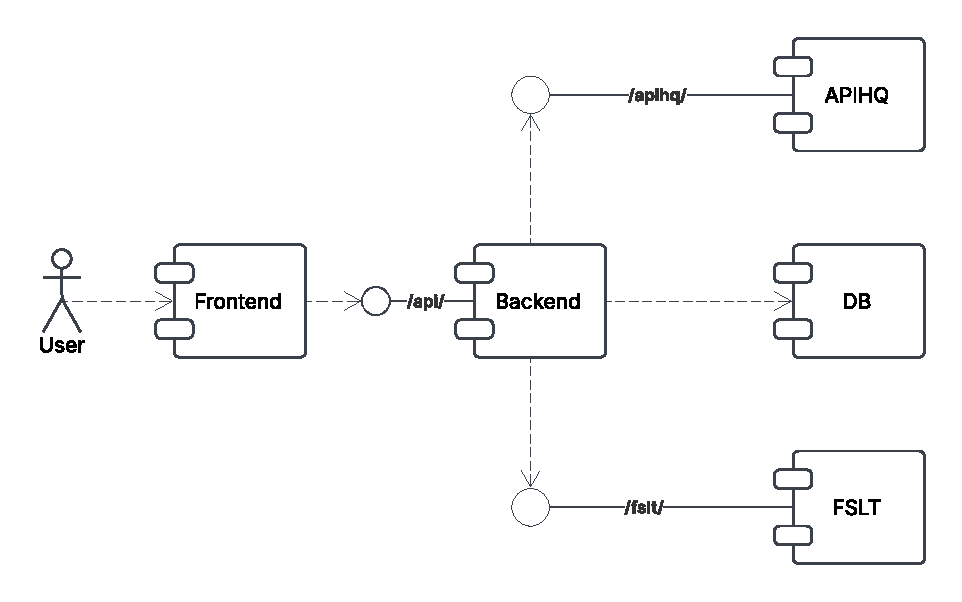
\includegraphics[width=\textwidth]{figures/components.pdf}
    \caption{Diagramma dell'architettura logica di sistema, che illustra i componenti principali e i loro flussi di interazione.}
    \label{fig:logical_architecture_diagram}
\end{figure}



\section{Design del Backend}
\label{sec:design_backend_oop}

Il componente backend rappresenta il nucleo logico dell'intera applicazione. La sua progettazione è stata affrontata con un approccio orientato agli oggetti, con l'obiettivo di creare un sistema modulare e facilmente estensibile. Per raggiungere tale scopo, sono state effettuate scelte di design mirate, partendo dalla definizione di un'architettura di alto livello fino all'applicazione di pattern specifici per risolvere le problematiche emerse durante la fase di analisi.

\subsection{Architettura a Strati per la Separazione delle Responsabilità}
\label{subsec:design_layered}

\paragraph{Problema di Design}
Un'applicazione web complessa deve gestire diverse responsabilità: interpretare le richieste HTTP, eseguire la logica di business e interagire con un sistema di persistenza dati. Senza una struttura chiara, queste responsabilità tendono a mescolarsi, creando un codice monolitico, difficile da comprendere, testare e manutenere. Questo fenomeno, noto come alto accoppiamento e bassa coesione, rende qualsiasi modifica futura rischiosa e costosa.

\paragraph{Soluzione di Design}
Per risolvere questo problema, il design del backend adotta il pattern architetturale \textbf{Layered Architecture} (Architettura a Strati). Questo pattern scompone l'applicazione in due tipologie di componenti: un insieme di strati orizzontali con responsabilità comportamentali, e un layer trasversale che contiene i modelli dei dati.

\paragraph{Model Layer (Strato dei Modelli Dati)}
Questo non è uno strato comportamentale, ma un componente trasversale che definisce gli oggetti di dominio e le strutture dati dell'applicazione. È utilizzato da tutti gli altri strati. Il design distingue due tipi di modelli:
\begin{itemize}
    \item Le \textbf{Entità del Dominio} che rappresentano i dati nel loro stato più puro e strutturato. Contengono la "verità" del sistema e vengono utilizzate principalmente dal Service Layer e dal Data Access Layer.
    \item I \textbf{Data Transfer Objects (DTO)}, che fungono da "contratto" dati per la comunicazione con l'esterno (il frontend) o tra gli strati stessi. Sono strutture dati semplici, ottimizzate per il trasferimento e spesso modellate per nascondere o aggregare i dati delle entità sottostanti.
\end{itemize}

\paragraph{Strati Comportamentali}
Gli strati che contengono la logica applicativa sono tre e comunicano in modo rigorosamente unidirezionale (dall'alto verso il basso):

\begin{itemize}
    \item \textbf{Presentation Layer (Strato di Presentazione):} È il punto di ingresso dell'applicazione. La sua unica responsabilità è quella di gestire la comunicazione HTTP. Riceve le richieste, valida e mappa i dati in ingresso in \textit{Data Transfer Objects (DTO)} e li passa allo strato di servizio. Al ritorno, riceve i DTO dal Service Layer e li serializza nella risposta HTTP. In questo progetto, questo strato è rappresentato dai \textit{Controller}.

    \item \textbf{Service Layer (Strato di Servizio):} Rappresenta il cuore dell'applicazione. Contiene tutta la logica di business e orchestra le operazioni. Opera sulle \textit{Entità} del dominio, applica le regole di business e coordina le interazioni con il Data Access Layer. È completamente agnostico rispetto al protocollo HTTP o alla fonte di persistenza.

    \item \textbf{Data Access Layer (Strato di Accesso ai Dati):} La sua unica responsabilità è la comunicazione con il database. Incapsula tutta la logica per mappare le \textit{Entità} del dominio da e verso le tabelle del database. In questo progetto, tale strato è implementato tramite il \textbf{Repository Pattern}.
\end{itemize}

Questa struttura garantisce un basso accoppiamento e un'alta coesione, rendendo il sistema più testabile (ogni strato può essere testato in isolamento, mockando le sue dipendenze) e più facile da manutenere ed estendere.

\begin{figure}[H]
    \centering
    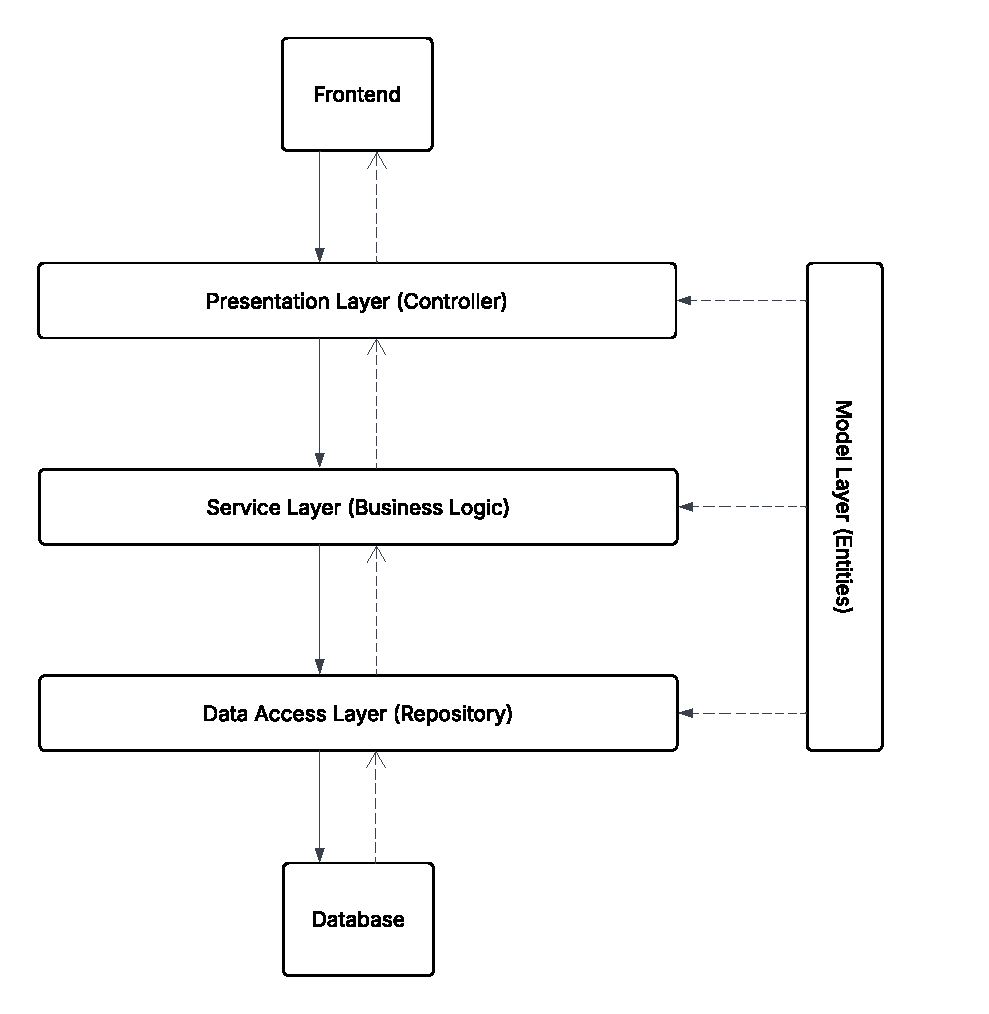
\includegraphics[width=0.7\textwidth]{figures/layer_design.pdf}
    \caption{Diagramma che illustra l'architettura a tre strati del backend e il flusso di comunicazione unidirezionale.}
    \label{fig:layered_architecture_uml}
\end{figure}

\subsection{Pattern Factory Method per la Creazione di Filtri Gateway}
\label{subsec:design_factory}

\paragraph{Problema di Design}
Dall'analisi delle integrazioni (Sezione \ref{sec:analisi_contesto}) è emersa la necessità di arricchire le richieste inoltrate ai due diversi endpoint esterni (API HQ e API Principale) con meccanismi di autenticazione differenti (Basic Auth per uno, API Key per l'altro). La sfida di design consisteva nel trovare un modo flessibile ed estensibile per creare e applicare queste logiche di modifica delle richieste in modo dinamico e disaccoppiato dalla configurazione delle rotte.


\paragraph{Soluzione di Design}
Per risolvere questo problema, è stato adottato il pattern creazionale Factory Method. Il design prevede la definizione di una interfaccia o classe base astratta, la \texttt{GatewayFilterFactory}, che dichiara un "metodo fabbrica" (\textit{factory method}) per la creazione di oggetti di tipo \texttt{GatewayFilter}. Un \texttt{GatewayFilter} è un oggetto la cui responsabilità è intercettare e modificare una richiesta HTTP.

Il design si completa con la creazione di due classi "fabbrica" concrete:
\begin{itemize}
    \item \texttt{ApiHqAuthGatewayFilterFactory}: Una fabbrica concreta che implementa il factory method per produrre un'istanza di \texttt{GatewayFilter} specializzata nell'aggiungere l'header di autenticazione Basic Auth, necessario per le chiamate verso l'endpoint API HQ.
    \item \texttt{FsfltApiKeyGatewayFilterFactory}: Un'altra fabbrica concreta il cui factory method produce un'istanza di \texttt{GatewayFilter} che si occupa di recuperare la chiave API dell'utente autenticato e di inserirla in un header specifico per le chiamate verso l'API Principale.
\end{itemize}


\begin{figure}[H]
    \centering
    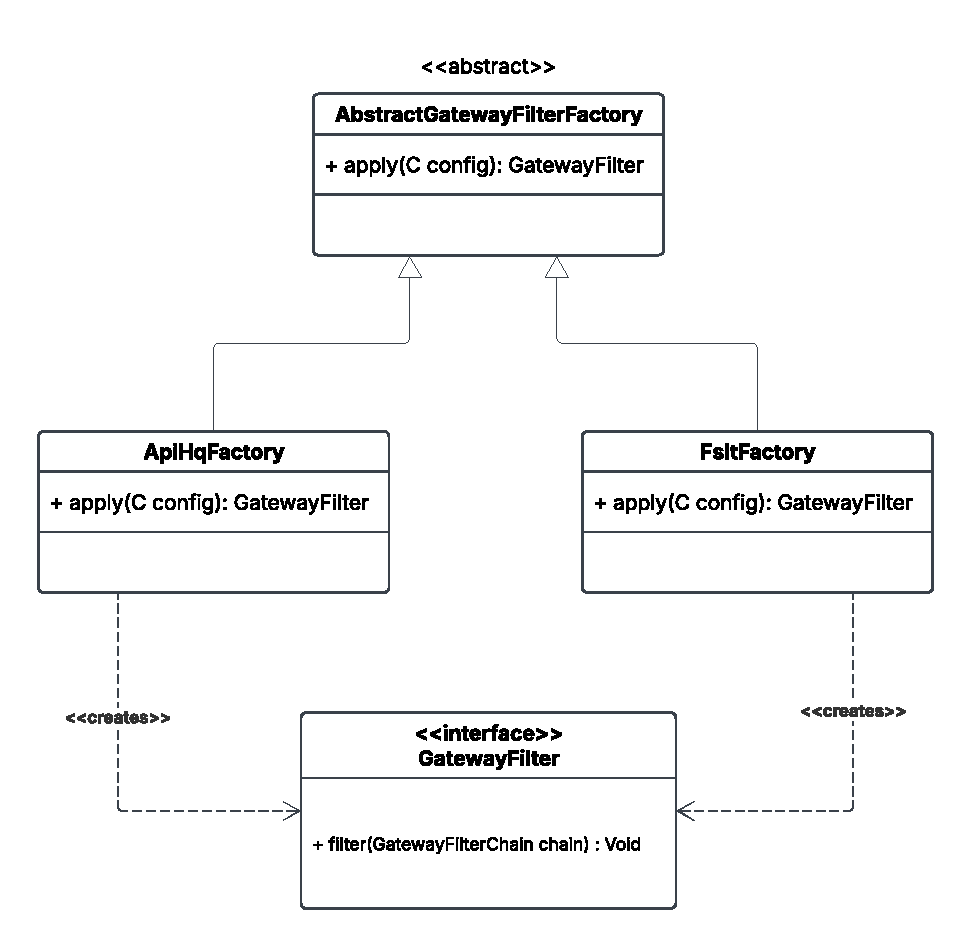
\includegraphics[width=0.8\textwidth]{figures/gwfactory.pdf}
    \caption{Diagramma delle classi che illustra l'applicazione del pattern Factory Method per la creazione dei filtri del gateway.}
    \label{fig:factory_method_uml}
\end{figure}

Questo approccio delega la responsabilità dell'istanziazione dei filtri alle sottoclassi, permettendo al sistema principale di configurazione delle rotte di operare a un alto livello di astrazione, senza conoscere i dettagli concreti di ciascun filtro. Ciò aumenta la modularità e semplifica l'eventuale aggiunta di nuovi filtri in futuro.



\subsection{Pattern Singleton per la Gestione dei Servizi}
\label{subsec:design_singleton}

\paragraph{Problema di Design}
Molti componenti del backend, come i servizi per la gestione della logica di business (es. autenticazione, generazione JWT) o i repository per l'accesso ai dati, sono intrinsecamente \textit{stateless} (privi di stato di istanza). La creazione di più istanze di tali oggetti sarebbe inefficiente e potrebbe portare a comportamenti anomali, rendendo necessaria una strategia per garantire che esista una e una sola istanza di questi componenti per tutta l'applicazione.

\paragraph{Soluzione di Design}
Per questo requisito, il design adotta il pattern Singleton. Tuttavia, invece di ricorrere a un'implementazione manuale e statica del pattern, che può introdurre rigidità e problemi di testabilità, il design prevede di delegare la gestione del ciclo di vita di questi oggetti a un componente infrastrutturale basato sul principio di Inversion of Control (IoC).

Secondo questo approccio, i componenti di servizio (come quelli per l'autenticazione o la generazione di token) e di accesso ai dati vengono registrati presso un gestore centrale. Sarà responsabilità di questo gestore istanziarli una sola volta (garantendo l'unicità del Singleton) e fornire tale istanza a qualsiasi altro componente che ne dichiari una dipendenza. Questo meccanismo, noto anche come Dependency Injection, permette ai componenti di essere ignari dei dettagli di creazione e del ciclo di vita delle proprie dipendenze.

\subsection{Pattern Facade per l'Autenticazione e la Gestione delle Sessioni}
\label{subsec:design_facade}

\paragraph{Problema di Design}
Il processo di autenticazione e gestione delle sessioni utente, per sua natura, è un'operazione complessa che richiede la coordinazione di molteplici componenti. Un client che volesse eseguire l'autenticazione dovrebbe interagire con un gestore degli utenti, un componente per la validazione delle credenziali, un servizio per la creazione dei token e un servizio per la gestione della sessione, dei quali molteplici interagiscono anche con il componente di persistenza dati. Esporre questa complessa rete di collaborazioni al client (in questo caso, il layer dei Controller) creerebbe un forte accoppiamento e renderebbe il codice difficile da comprendere, utilizzare e manutenere.

\paragraph{Soluzione di Design}
Per nascondere questa complessità e fornire un punto di accesso unificato e semplice, è stato applicato il pattern strutturale Facade. Il design prevede la creazione di una classe \texttt{AuthenticationService} che agisce, per l'appunto, da "facciata" per l'intero sottosistema di autenticazione.

Questa classe espone un set di metodi ad alto livello, come \texttt{autentica\allowbreak Utente\allowbreak (...)} o \texttt{ruota\allowbreak Refresh\allowbreak Token\allowbreak (...)}. Al suo interno, la facciata orchestra le chiamate ai vari componenti del sottosistema (il repository degli utenti, il gestore dei token, il validatore delle password, etc.), ma nasconde completamente questi dettagli di interazione al chiamante. In questo modo, il client (il \texttt{Auth\allowbreak Controller}) dipende unicamente dall'interfaccia semplificata della Facade, risultando completamente disaccoppiato dalla logica interna del sottosistema. Questo non solo semplifica il codice del client, ma permette anche di modificare e far evolvere il sottosistema di autenticazione in modo indipendente, senza impattare il resto dell'applicazione.

\begin{figure}[H]
    \centering
    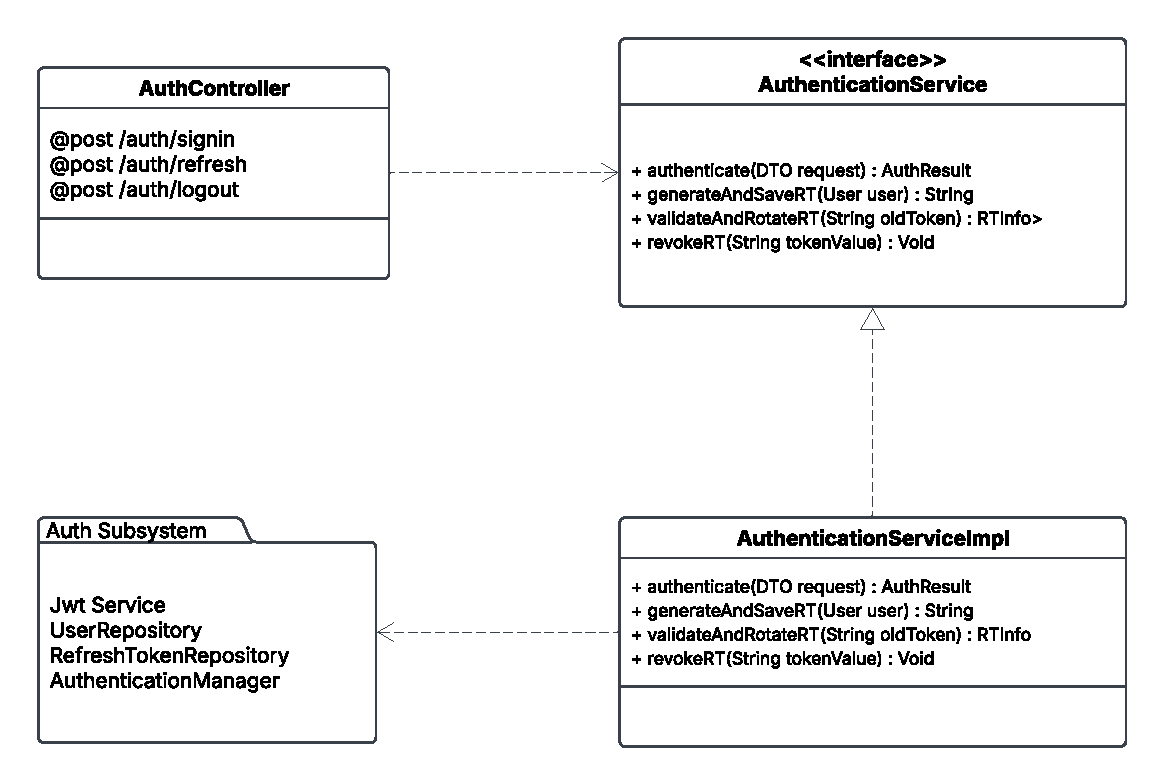
\includegraphics[width=0.9\textwidth]{figures/facade.pdf}
    \caption{Diagramma delle classi che mostra come \texttt{AuthenticationService} agisca da Facade, semplificando l'accesso al sottosistema di autenticazione.}
    \label{fig:facade_uml}
\end{figure}

\subsection{Pattern Data Transfer Object (DTO) per lo Scambio di Dati}
\label{subsec:design_dto}

\paragraph{Problema di Design}
La comunicazione tra i diversi layer dell'applicazione (es. tra Controller e Service) e, soprattutto, tra il backend e il client frontend, richiede uno scambio di dati strutturati. Utilizzare direttamente gli oggetti del dominio (le "entità" che rappresentano i dati nel database, come \texttt{User} o \texttt{RefreshToken}) per questo scopo è una pratica sconsigliata. Esporre il modello di dominio interno potrebbe rivelare dettagli implementativi, creare dipendenze indesiderate e introdurre vulnerabilità di sicurezza, oltre a rendere l'API rigida e difficile da far evolvere.

\paragraph{Soluzione di Design}
Per risolvere questo problema di disaccoppiamento e sicurezza, è stato adottato il pattern Data Transfer Object (DTO). Il design prevede la creazione di un insieme di classi semplici, il cui unico scopo è quello di fungere da contenitori di dati (data carrier) per le informazioni scambiate attraverso i confini dell'API.

Per esempio, per una richiesta di autenticazione, il client non invia un oggetto di dominio, ma un \texttt{AuthRequestDTO} contenente solo i campi strettamente necessari (email e password). Analogamente, la risposta del backend non sarà l'oggetto \texttt{User} completo, ma un \texttt{AuthResponseDTO} contenente solo il token di accesso e le informazioni sulla sua scadenza.

Questo approccio offre molteplici vantaggi:
\begin{itemize}
    \item \textbf{Disaccoppiamento}: Il modello dati dell'API (i DTO) è indipendente dal modello dati di persistenza (le entità). È possibile modificare la struttura del database senza impattare i client dell'API.
    \item \textbf{Sicurezza}: Vengono esposti solo i dati strettamente necessari, nascondendo informazioni sensibili (come le password hashate o altri dati interni dell'entità \texttt{User}).
    \item \textbf{Ottimizzazione}: I DTO possono essere modellati per aggregare dati provenienti da più entità, riducendo il numero di chiamate necessarie al client per ottenere le informazioni di cui ha bisogno.
\end{itemize}

L'uso dei DTO definisce un "contratto" chiaro e stabile per le API, fondamentale per un'architettura a servizi in cui frontend e backend evolvono in modo indipendente.

\section{Design del Frontend}
\label{sec:design_frontend}

Sebbene il paradigma dominante nello sviluppo con React sia funzionale/dichiarativo, i principi fondamentali della programmazione orientata agli oggetti -- come l'incapsulamento, la composizione e la separazione delle responsabilità -- sono stati la guida per la progettazione del frontend. L'obiettivo era creare un'architettura a componenti che fosse non solo reattiva e performante, ma anche logicamente strutturata e scalabile.

\subsection{Architettura a Componenti come Composizione di Oggetti}
\label{subsec:design_component_composition}

\paragraph{Problema di Design}
La costruzione di un'interfaccia utente complessa e interattiva come quella richiesta rischia di portare a un codice monolitico, difficile da comprendere, testare e far evolvere. Era necessario un approccio che permettesse di gestire la complessità attraverso la decomposizione.

\paragraph{Soluzione di Design}
Il design del frontend si basa su un'architettura a componenti, che è l'analogo del principio di composizione nella programmazione orientata agli oggetti. L'interfaccia utente è stata scomposta in una gerarchia di componenti React, ciascuno dei quali può essere visto come un "oggetto" con le proprie proprietà (\textit{props}), il proprio stato interno (\textit{state}) e il proprio comportamento (metodi e gestori di eventi).

Questo approccio ha permesso di distinguere due tipologie di componenti:
\begin{itemize}
    \item \textbf{Componenti "Container" (o Smart)}: Hanno la responsabilità di gestire la logica e lo stato. Si occupano di recuperare i dati (interagendo con i servizi API) e di passarli ai componenti sottostanti.
    \item \textbf{Componenti "Presentazionali" (o Dumb)}: La loro unica responsabilità è quella di visualizzare i dati ricevuti tramite \textit{props} e di notificare ai componenti genitori eventuali interazioni dell'utente. Sono altamente riutilizzabili.
\end{itemize}

\subsection{Pattern Strategy per Componenti Configurabili}
\label{subsec:design_strategy_frontend}

\paragraph{Problema di Design}
La dashboard (pagina Home) richiede la visualizzazione di molteplici grafici. Sebbene ogni grafico abbia una logica di base simile (titolo, selettore temporale, recupero dati, gestione del caricamento), ognuno di essi si differenzia per l'endpoint da interrogare, la trasformazione da applicare ai dati e le opzioni di visualizzazione (es. grafico a barre vs. grafico a torta). Creare un componente specifico per ogni grafico avrebbe comportato una notevole duplicazione di codice.

\paragraph{Soluzione di Design}
Per risolvere questo problema in modo elegante, è stato applicato un design che ricalca il pattern Strategy. È stato progettato un singolo componente generico, \texttt{GenericChart}, che agisce come "contesto". Questo componente non contiene la logica specifica di nessun grafico, ma è progettato per ricevere un oggetto \texttt{config} tramite le sue \textit{props}.

Questo oggetto di configurazione definisce la "strategia" completa per un particolare grafico: l'endpoint da chiamare, i parametri della query, la funzione per trasformare la risposta dell'API in un formato compatibile con la libreria di grafici, e le opzioni di rendering. Le diverse strategie sono definite centralmente nel file \texttt{chartConfigs.ts}. In questo modo, per renderizzare un nuovo tipo di grafico è sufficiente definire una nuova strategia, senza modificare il componente \texttt{GenericChart}, promuovendo i principi di Open/Closed e di riuso del software.

\begin{figure}[H]
    \centering
    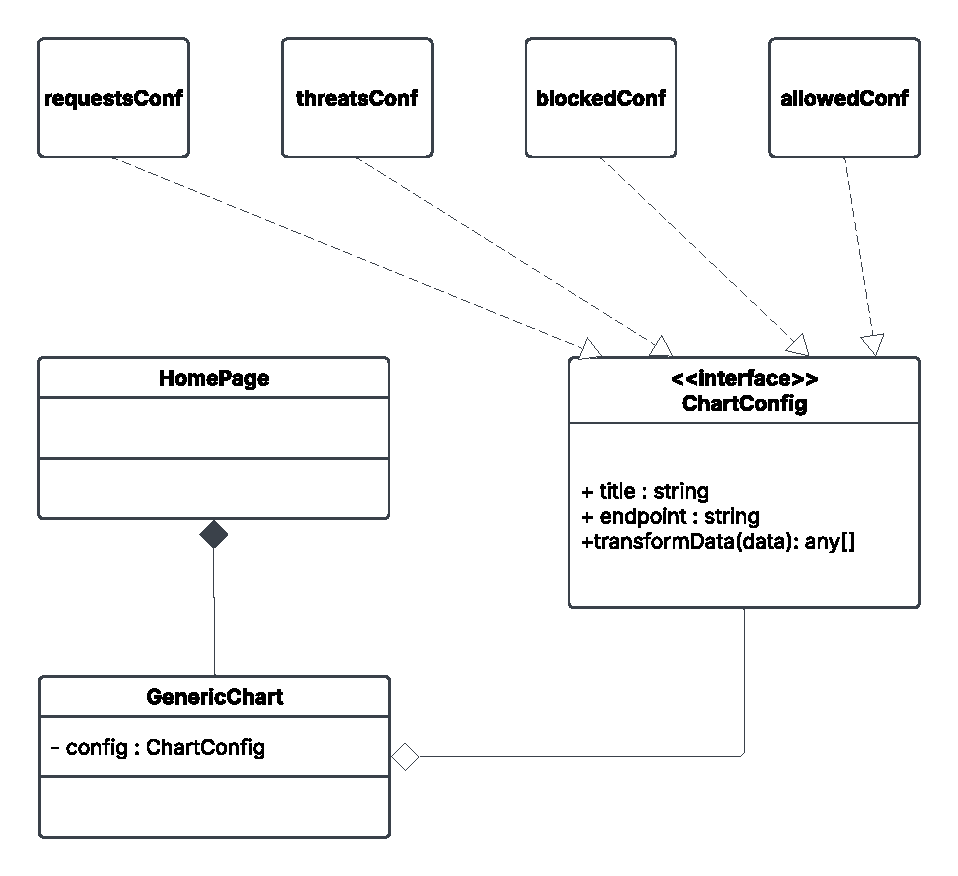
\includegraphics[width=\textwidth]{figures/strategy.pdf}
    \caption{Diagramma che illustra come il componente \texttt{GenericChart} utilizzi diversi oggetti \texttt{ChartConfig} (strategie) per renderizzare grafici differenti.}
    \label{fig:strategy_frontend_uml}
\end{figure}



\subsection{Gestione dello Stato Globale con il Pattern Observer}
\label{subsec:design_observer_frontend}

\paragraph{Problema di Design}
In un'applicazione complessa, numerosi componenti distribuiti nell'albero della UI necessitano di accedere e reagire a cambiamenti di uno stesso stato condiviso. Esempi tipici in questo progetto sono lo stato di autenticazione dell'utente o il codice del cliente e del profilo attualmente selezionati. Far transitare questi dati attraverso l'intera gerarchia di componenti tramite le \textit{props} (una pratica nota come "prop drilling") è inefficiente, crea un forte accoppiamento tra i componenti e rende l'applicazione estremamente rigida e difficile da manutenere.

\paragraph{Soluzione di Design}
Per risolvere questo problema di gestione dello stato globale in modo pulito e scalabile, il design adotta un'architettura che ricalca il pattern comportamentale Observer. La soluzione prevede la creazione di "soggetti" osservabili centralizzati (\textit{subjects}), denominati \texttt{AuthProvider} e \texttt{CustomerProvider}, che detengono lo stato condiviso.

I componenti che necessitano di accedere a questo stato agiscono come "osservatori" (\textit{observers}), "sottoscrivendo" l'interesse verso le notifiche di cambiamento tramite un meccanismo di accesso al contesto (i custom hook \texttt{useAuth} e \texttt{useCustomer}). Quando lo stato in un \textit{provider} cambia (ad esempio, l'utente effettua il logout o seleziona un nuovo cliente), il \textit{provider} notifica automaticamente tutti i componenti sottoscrittori, che possono così reagire e aggiornare la propria vista di conseguenza. Questo design disaccoppia efficacemente i componenti, che non necessitano di una comunicazione diretta, ma reagiscono in modo indipendente ai cambiamenti di uno stato centralizzato.

\subsection{Centralizzazione delle Chiamate API (Singleton e Decorator)}
\label{subsec:design_api_singleton_decorator}

\paragraph{Problema di Design}
Le chiamate asincrone verso il backend sono una responsabilità trasversale a molti componenti. Ogni chiamata deve includere il token di autenticazione e deve gestire correttamente la possibile scadenza di tale token, avviando un flusso di rinnovo. Implementare questa logica in ogni singolo componente che recupera dati porterebbe a una massiccia duplicazione di codice e a una manutenibilità quasi nulla.

\paragraph{Soluzione di Design}
Il design affronta questo problema attraverso la creazione di un servizio API centralizzato. Viene definita una singola istanza di un client HTTP, configurata per l'intera applicazione, che agisce come un Singleton. Questo garantisce che tutte le impostazioni di comunicazione (come l'URL di base o i timeout) siano coerenti.

Su questa istanza unica, viene applicato un pattern riconducibile al Decorator, utilizzando il meccanismo degli "intercettori".
\begin{itemize}
    \item \textbf{Intercettore di Richiesta}: "Decora" ogni richiesta in uscita, aggiungendo dinamicamente l'header \texttt{Authorization} con il token JWT dell'utente. I componenti che effettuano la chiamata non devono preoccuparsi di questo dettaglio.
    \item \textbf{Intercettore di Risposta}: "Decora" la gestione degli errori, intercettando specificamente le risposte di tipo \texttt{401 Unauthorized} (token scaduto). In questo caso, l'intercettore gestisce in modo trasparente l'intero flusso di rinnovo del token, mettendo in pausa la richiesta originale, ottenendo un nuovo token e, infine, ripetendo la richiesta fallita con le nuove credenziali.
\end{itemize}
Questo design a strati astrae completamente la complessità della comunicazione autenticata, lasciando ai componenti della UI la sola responsabilità di richiedere i dati di cui hanno bisogno.

\chapter{Implementazione}
\label{chap:implementazione}

Questo capitolo illustra come i principi e le architetture definiti nel capitolo \ref{chap:design} siano stati tradotti in scelte tecnologiche concrete e codice sorgente. L'obiettivo è dimostrare come le decisioni di progettazione abbiano guidato la selezione e l'utilizzo dello stack tecnologico per realizzare gli obiettivi del progetto.

\section{Traduzione del Design in Scelte Tecnologiche}
\label{sec:impl_tech_choices}

La fase implementativa ha richiesto di selezionare gli strumenti più adatti a realizzare l'architettura a strati, i pattern di comunicazione e la gestione dello stato delineati nel design.

\subsection{Backend: la Scelta di un Ecosistema Reattivo con Spring WebFlux}
Il design del backend (Sezione \ref{sec:design_backend_oop}) richiedeva un'architettura a strati robusta, la gestione di servizi stateless (Singleton) e, soprattutto, la capacità di gestire in modo efficiente un alto numero di operazioni di I/O concorrenti, data la necessità di interfacciarsi con API esterne.

Per tradurre questi requisiti in una soluzione concreta, la scelta è ricaduta sull'ecosistema \textit{Java} e sul framework \textit{Spring Boot}. Java offre robustezza e un ecosistema maturo, mentre Spring Boot fornisce un potente meccanismo di \textit{Inversion of Control (IoC)} e \textit{Dependency Injection}, che rappresenta l'implementazione pratica perfetta per il design basato sul pattern Singleton per la gestione dei servizi, astraendo completamente lo sviluppatore dalla loro creazione e dal loro ciclo di vita.

Tuttavia, per ovvire al problema dell'I/O concorrente, si è fatta una scelta implementativa fondamentale: adottare il paradigma di programmazione reattiva. All'interno dell'ecosistema Spring, questo ha significato scegliere Spring WebFlux al posto del tradizionale Spring MVC. Questa scelta permette di realizzare un backend non bloccante, che è la soluzione tecnica ideale per un'applicazione il cui carico di lavoro è dominato da attese di rete. Per mantenere la coerenza del modello reattivo end-to-end, anche per l'accesso ai dati è stata fatta una scelta conseguente: utilizzare Spring Data R2DBC invece del classico JDBC, garantendo che nessuna operazione, neanche sul database, potesse bloccare i thread principali dell'applicazione.

\subsection{Frontend: Realizzazione dei Pattern di Design con React e Axios}
Il design del frontend (Sezione \ref{sec:design_frontend}) prevedeva un'architettura a componenti, una gestione centralizzata dello stato (pattern Observer) e un meccanismo robusto e centralizzato per la comunicazione con le API (pattern Singleton e Decorator).

\paragraph{Componenti e Stato}
Il design basato sulla composizione di oggetti è stato implementato utilizzando la libreria React, come dettato dal requisito non funzionale \ref{req:comformity}. La sua architettura nativamente basata su componenti ha permesso di tradurre direttamente il design di componenti "Container" e "Presentazionali". Per realizzare il pattern Observer per la gestione dello stato globale, si è scelto di utilizzare la React Context API. Questa soluzione, interna a React, è stata preferita a librerie esterne più complesse (come Redux) perché offriva il livello di funzionalità necessario per il progetto (sottoscrizione e notifica dei cambiamenti di stato) in modo più semplice e integrato.

\paragraph{Comunicazione API Centralizzata}
Il design di un punto di accesso unico e decorato per le chiamate API ha guidato la scelta e l'utilizzo della libreria Axios. Per implementare il pattern Singleton, è stata creata un'unica istanza configurata di Axios (\texttt{axiosInstance.ts}), esportata e utilizzata in tutta l'applicazione. Il pattern Decorator è stato realizzato sfruttando la funzionalità nativa degli intercettori di Axios. Sono stati configurati due intercettori:
\begin{itemize}
    \item Un \textit{intercettore di richiesta}, che "decora" ogni chiamata in uscita aggiungendo dinamicamente l'header di autenticazione \texttt{Authorization}.
    \item Un \textit{intercettore di risposta}, che "decora" la gestione degli errori intercettando le risposte \texttt{401 Unauthorized} per avviare in modo trasparente il flusso di rinnovo del token.
\end{itemize}

\paragraph{Struttura dell'Interfaccia Utente e Navigazione}
L'applicazione segue il modello di una Single Page Application (SPA), dove la navigazione tra le diverse aree funzionali avviene senza ricaricare la pagina, garantendo un'esperienza utente fluida. La logica di navigazione è gestita dalla libreria React Router, che mappa i percorsi dell'URL ai componenti React corrispondenti.

L'interfaccia è stata scomposta in quattro schermate principali, ognuna rappresentata da un componente "vista" di alto livello:
\begin{itemize}
    \item \textbf{Pagina di Login:} Il punto di accesso all'applicazione, responsabile della raccolta delle credenziali e della gestione del processo di autenticazione.
    \item \textbf{Dashboard Principale:} La schermata di atterraggio dopo il login. Presenta una panoramica dei dati più importanti tramite una serie di grafici e widget informativi, offrendo una visione d'insieme immediata.
    \item \textbf{Vista delle Policy di Protezione:} Una sezione dedicata alla consultazione in sola lettura delle policy di filtraggio attive, delle liste di domini (blacklist/whitelist) e delle altre configurazioni di sicurezza.
    \item \textbf{Pagina di Ricerca Dominio (Lookup):} Uno strumento che permette all'utente di interrogare un dominio specifico per verificare come viene classificato e gestito dal sistema di filtraggio.
\end{itemize}
Ogni schermata è a sua volta composta da componenti più piccoli e riutilizzabili, seguendo una chiara gerarchia che separa la logica di recupero dati (nei componenti "container") dalla logica di pura presentazione.

\begin{figure}[H]
    \centering
    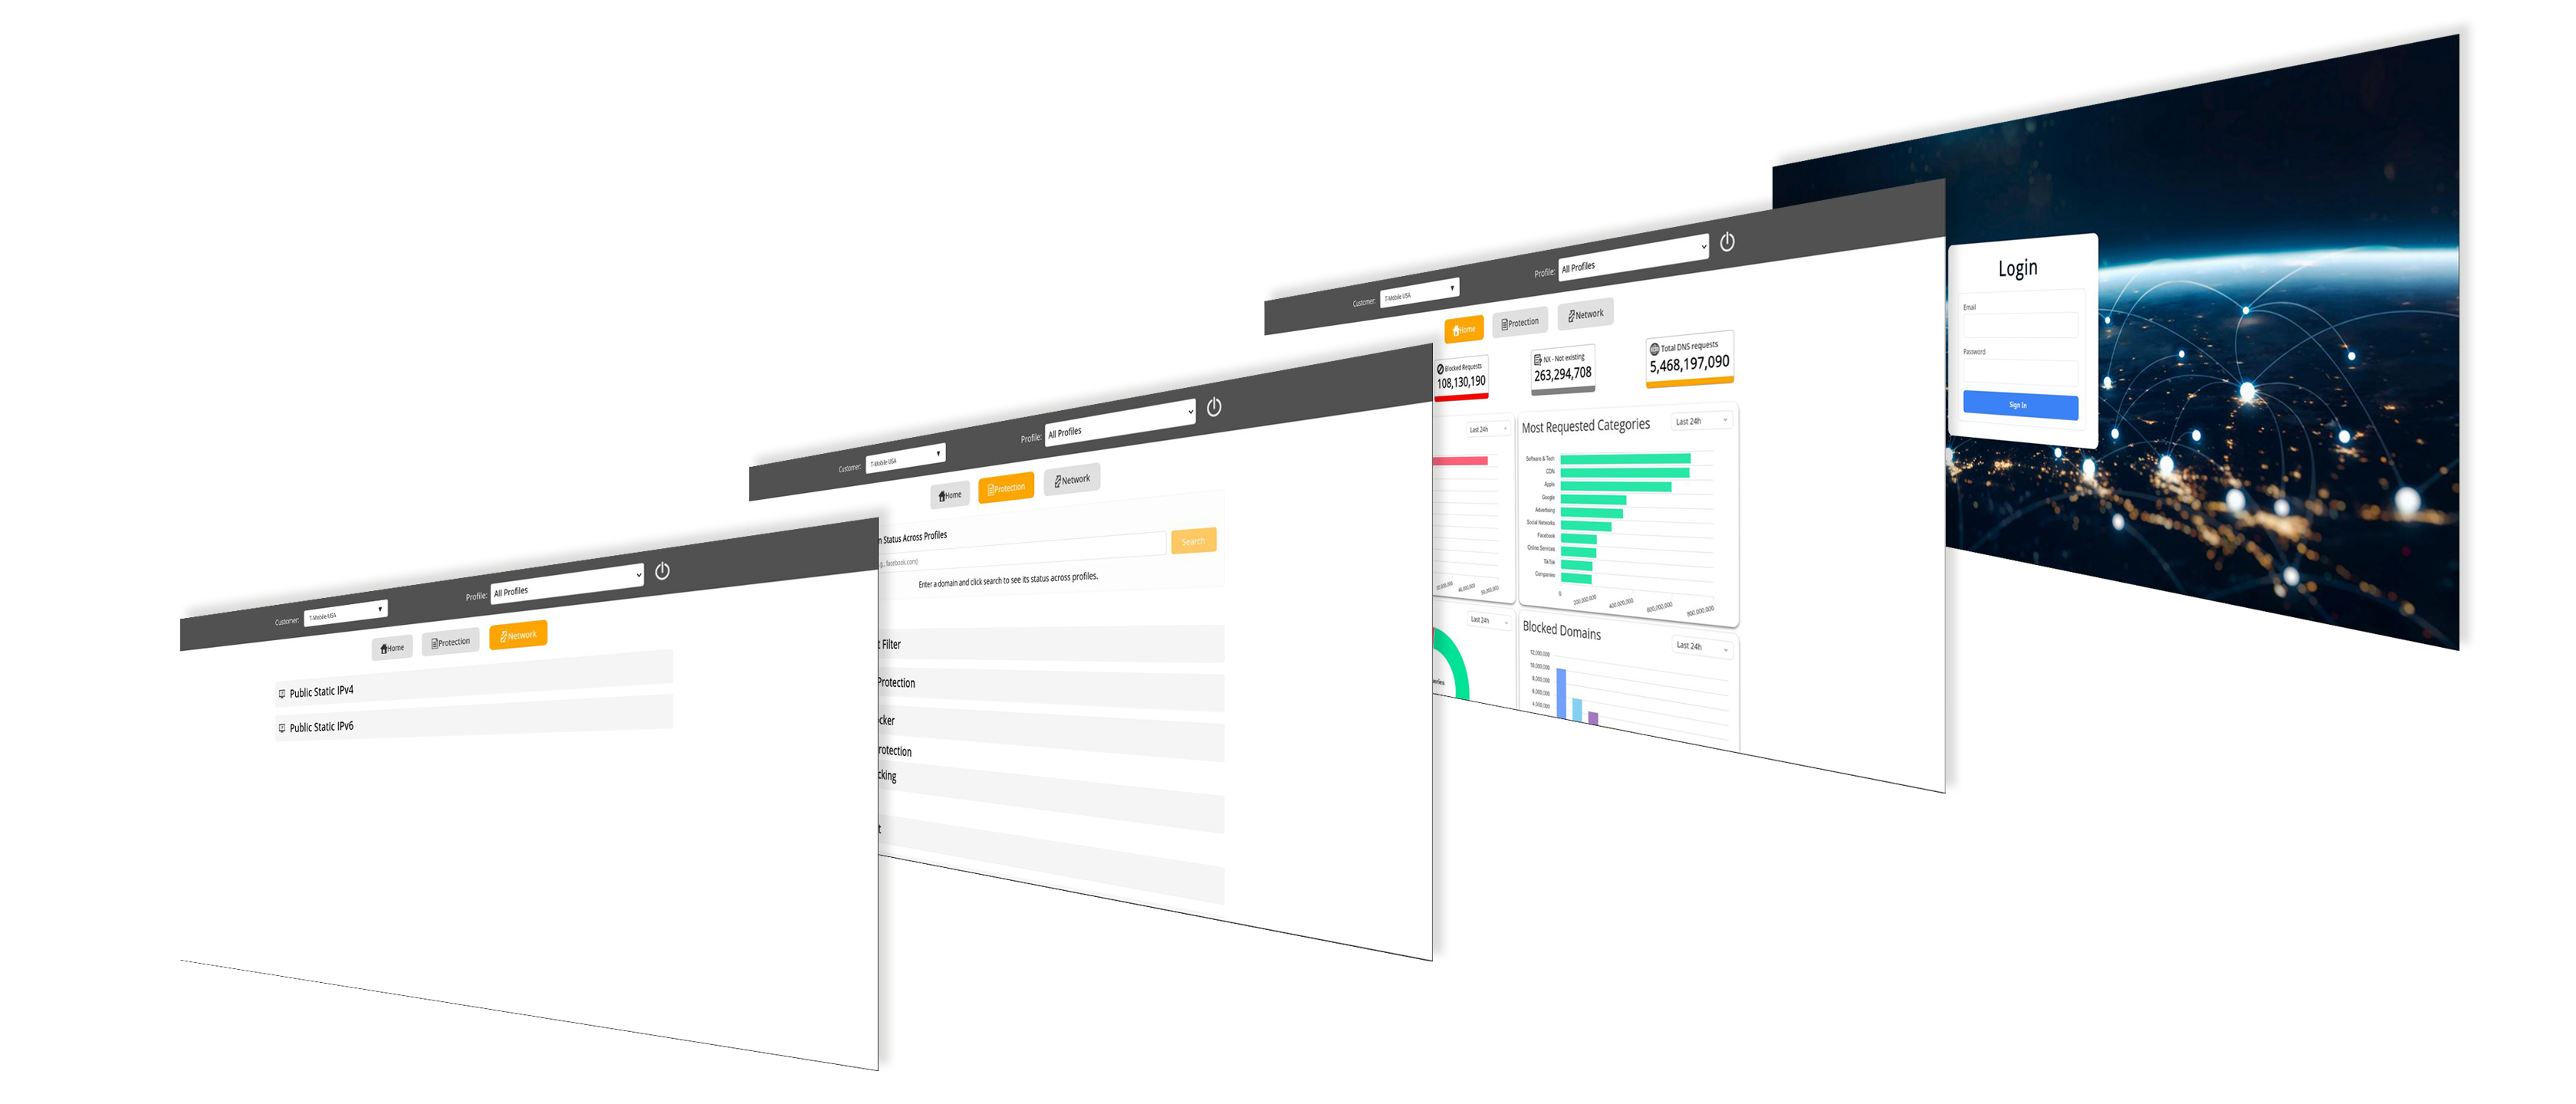
\includegraphics[width=\textwidth]{figures/slideshow.png}
    \caption{Panoramica delle schermate principali dell'applicazione frontend: la pagina di Login, la Dashboard principale con i grafici, la vista delle Policy di protezione e la funzionalità di analisi dei domini.}
    \label{fig:ui_screens}
\end{figure}

\section{Implementazione del Flusso di Sicurezza End-to-End}
\label{sec:impl_security}

Questa sezione descrive la realizzazione pratica del flusso di sicurezza, traducendo il design concettuale in componenti software specifici sia nel backend che nel frontend. Il sistema implementa un'autenticazione stateless basata su JSON Web Tokens (JWT) con un meccanismo di rotazione per i refresh token, come conseguenza del requisito \ref{req:security}.
e.

\paragraph{Generazione dei Token e Gestione dei Cookie}
Al momento del login, l' \texttt{Auth\allowbreak Controller} riceve le credenziali e le delega all' \texttt{Authentication\allowbreak Service}. Questo servizio, agendo come Facade, orchestra la validazione e, in caso di successo, invoca un \texttt{Jwt\allowbreak Service} dedicato. Questa classe utilizza la libreria \texttt{io.\allowbreak jsonwebtoken.\allowbreak jjwt} per creare e firmare i token.
\begin{itemize}
    \item L'\textbf{Access Token} viene generato come un JWT firmato, contenente i \textit{claims} dell'utente (username e ruoli) e una scadenza breve di 15 minuti.
    \item Il \textbf{Refresh Token} viene generato come stringa crittograficamente sicura e con una scadenza lunga (7 giorni). L'hash del token viene salvato nel database PostgreSQL tramite il \texttt{RefreshTokenRepository} per la validazione futura.
\end{itemize}
L' \texttt{AuthController} si occupa poi di inviare i token al client. L'Access Token viene restituito nel corpo della risposta JSON, mentre il Refresh Token viene inserito in un cookie. Per questa operazione si utilizza la classe helper \texttt{ResponseCookie} di Spring, che permette di configurare in modo dichiarativo gli attributi di sicurezza \texttt{HttpOnly}\footnote{L'attributo HttpOnly impedisce che il cookie possa essere letto tramite JavaScript. Fondamentale per mitigare attacchi di tipo Cross-Site Scripting (XSS), in cui uno script malevolo potrebbe tentare di rubare il token di sessione.}, \texttt{Secure} (i.e. utilizzare solo HTTPS), \texttt{Path} e \texttt{Max-Age}, garantendo che il refresh token sia protetto da accessi via JavaScript (XSS) e trasmesso solo su connessioni HTTPS.

\paragraph{Implementazione della Rotazione del Token}
Il cuore della sicurezza del sistema è implementato nel metodo \texttt{validateAndRotateRefreshToken} all'interno dell' \texttt{AuthenticationService}. Quando l'endpoint \texttt{/auth/refresh} viene chiamato, questo metodo esegue la logica di rotazione. L'intero processo è annotato con \texttt{@Transactional} di Spring, per assicurare che la ricerca, la cancellazione del vecchio token e il salvataggio del nuovo avvengano come una transazione atomica sul database, prevenendo condizioni di gara (\textit{race conditions}) e garantendo la consistenza dei dati. Se il token fornito è valido, viene immediatamente invalidato e sostituito, rendendolo a tutti gli effetti un token monouso per prevenire attacchi di tipo \textit{replay}.

\paragraph{Memorizzazione dell'Access Token e Gestione dello Stato}
In accordo con le best practice di sicurezza, l'Access Token non viene mai memorizzato nel \texttt{localStorage} o \texttt{sessionStorage}. Viene invece mantenuto esclusivamente nello stato in memoria dell'applicazione, gestito tramite un React Context (\texttt{AuthContext}). Questo minimizza l'esposizione del token a vulnerabilità di tipo Cross-Site Scripting. I componenti che effettuano chiamate API protette recuperano il token corrente dal contesto tramite un custom hook \texttt{useAuth()}.

\paragraph{Intercettore per il Rinnovo Automatico}
La logica di rinnovo è centralizzata in un intercettore configurato sull'istanza globale di Axios (\texttt{axiosInstance.ts}). Questo intercettore ispeziona ogni risposta proveniente dal server.
\begin{itemize}
    \item Se la risposta ha uno stato HTTP \texttt{401 Unauthorized}, l'intercettore "cattura" l'errore.
    \item Mette in pausa la richiesta originale fallita e avvia una nuova chiamata all'endpoint \texttt{/auth/refresh}. Essendo una normale richiesta HTTP, il browser allega automaticamente il cookie \texttt{HttpOnly} contenente il Refresh Token.
    \item In caso di successo, il nuovo Access Token viene salvato nel \texttt{AuthContext}, e la richiesta originale viene ritentata con il nuovo token.
    \item In caso di fallimento del refresh, l'utente viene disconnesso e reindirizzato alla pagina di login.
\end{itemize}
Questo approccio astrae completamente la complessità della gestione delle sessioni dai componenti della UI, che possono effettuare chiamate API senza doversi preoccupare della scadenza dei token.

\begin{figure}[H]
    \centering
    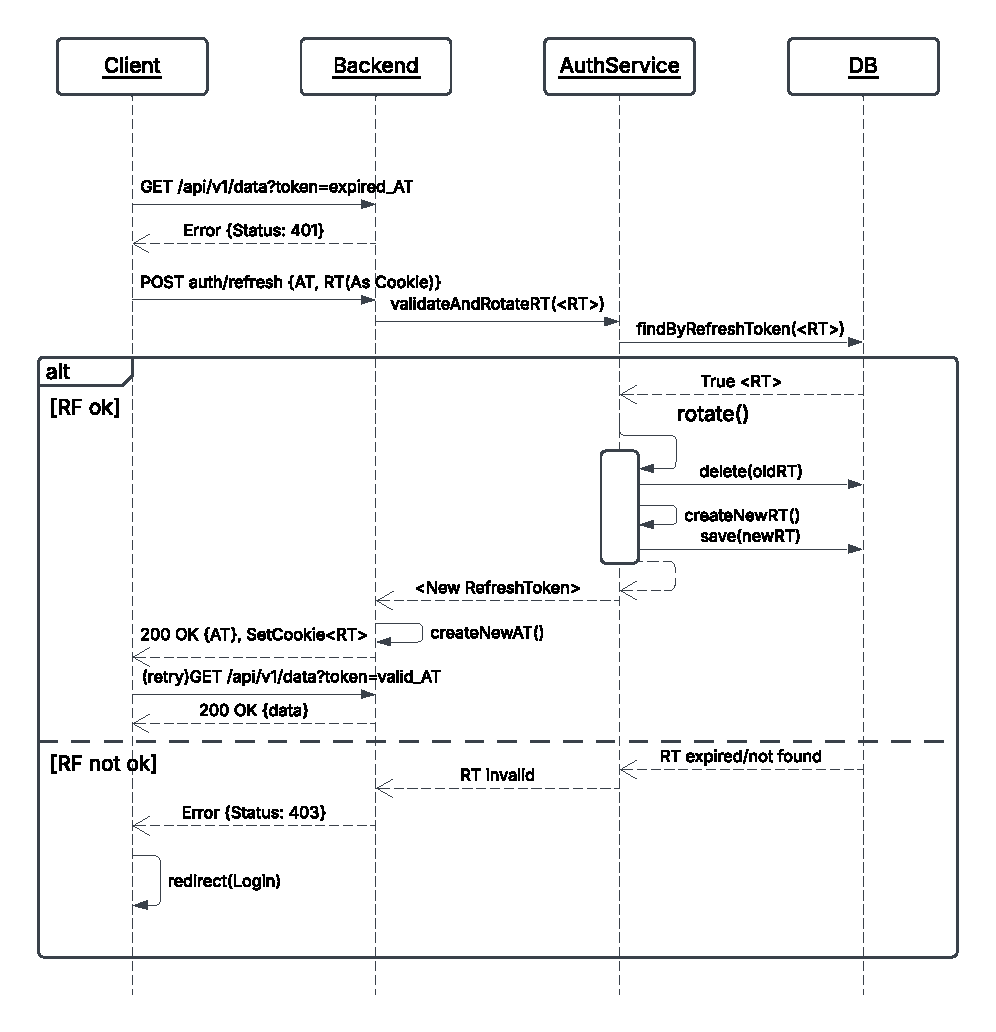
\includegraphics[width=\textwidth]{figures/expired_ac.pdf}
    \caption{Diagramma di sequenza che illustra il flusso di gestione di un Access Token scaduto e la rotazione del Refresh Token, evidenziando le interazioni tra client, backend e database.}
    \label{fig:token_rotation_sequence_uml}
\end{figure}


\chapter{Metodologia e Infrastruttura di Sviluppo}
\label{chap:metodologia}

Oltre alla progettazione e all'implementazione del software, un progetto di successo si basa su una solida metodologia di sviluppo e su un'infrastruttura di supporto affidabile. Questo capitolo descrive il processo operativo adottato per la realizzazione del progetto, dalla gestione agile alla strategia di testing, fino all'architettura della pipeline CI/CD che automatizza il rilascio dell'applicazione.

\section{Metodologia di Sviluppo Agile}
\label{sec:metodologia_agile}

Data la natura del progetto come "ponte tecnologico" e i vincoli temporali, si è scelto di non adottare un modello a cascata rigido, ma un approccio iterativo e incrementale, ispirato ai principi delle metodologie agili.

\paragraph{Collaborazione con gli Stakeholder} Lo sviluppo è avvenuto in stretta collaborazione con il \textit{product owner} e gli stakeholder aziendali di FlashStart. Questo ha garantito un allineamento costante con le esigenze del business e ha permesso di ricevere feedback tempestivi.

\paragraph{Iterazioni e Demo} Il lavoro è stato organizzato in cicli di sviluppo brevi, assimilabili a degli \textit{sprint}, della durata di circa una settimana (misurata in termini di ore di lavoro). Al termine di ogni ciclo, veniva presentata una demo dello stato di avanzamento del prodotto. Questo approccio ha permesso di:
\begin{itemize}
    \item Validare i requisiti in modo incrementale.
    \item Identificare e correggere eventuali incomprensioni o problemi in una fase precoce.
    \item Mantenere alta la visibilità del progetto all'interno dell'azienda, rafforzando la fiducia degli stakeholder.
\end{itemize}

\section{Strategia di Testing e Validazione}
\label{sec:testing}
Per garantire la qualità, la robustezza e la non regressione del software, è stata implementata una strategia di testing a più livelli, coprendo sia il backend che il frontend.

\subsection{Testing del Backend}
Per il backend sono state implementate due tipologie principali di test, sfruttando il framework di testing JUnit 5 e la libreria Mockito per la creazione di mock.

\paragraph{Unit Test} I test unitari si concentrano sulla verifica del comportamento di singole classi o metodi in isolamento. Un esempio tipico è la verifica dei servizi di autenticazione, dove le dipendenze esterne (come repository di dati e servizi di validazione) vengono sostituite con oggetti mock. Questo approccio permette di testare in modo isolato la logica di business critica, come la rotazione dei token, la validazione delle credenziali e la gestione degli errori, senza dipendere da risorse esterne come database o servizi di rete.

\paragraph{Integration Test} Per verificare l'interazione tra più componenti, come la logica di servizio e il layer di persistenza, sono stati scritti test di integrazione. Questi test utilizzano un database in-memory H2, configurato per emulare PostgreSQL, come specificato nel file di properties dei test. Ciò permette di testare il flusso completo di salvataggio e recupero dati (es. la creazione di un utente e del suo refresh token) in un ambiente controllato ma realistico.

\subsection{Testing del Frontend}
Per il frontend è stata utilizzata la libreria Jest. L'approccio si è concentrato sul testare i componenti dal punto di vista dell'utente.

\paragraph{Component Test} I test verificano che i componenti si renderizzino correttamente e rispondano alle interazioni dell'utente. Un esempio è il test per la pagina di Login, \texttt{Login.test.tsx}, che simula l'inserimento di testo da parte dell'utente, il click sul pulsante di submit e verifica che vengano mostrati i messaggi di errore o di successo appropriati.

\paragraph{Mocking delle Chiamate API} Per isolare i componenti frontend dal backend durante i test, le chiamate API effettuate sono state intercettate e simulate (mocking). 

\section{Deployment e Pipeline di CI/CD}
\label{sec:ci_cd}
Per automatizzare il processo di rilascio e garantire la coerenza degli ambienti, come richiesto da \ref{req:comformity}, è stata progettata e implementata una pipeline CI/CD.

\paragraph{Containerizzazione con Docker}
Il fondamento dell'infrastruttura è la containerizzazione. L'intera applicazione (frontend, backend, database) è definita come un insieme di servizi in un file \texttt{docker-compose.yaml}. Questo garantisce che ogni sviluppatore e ogni ambiente di deployment esegua il software con le stesse dipendenze e configurazioni. Sono state utilizzate build multi-stage nei Dockerfile per creare immagini finali ottimizzate e leggere, separando le dipendenze di build da quelle di runtime.

\paragraph{Pipeline Ibrida}
È stata scelta un'architettura di CI/CD ibrida, sfruttando i punti di forza di diverse tecnologie:
\begin{itemize}
    \item \textbf{GitHub Actions} viene utilizzato come orchestratore del flusso di lavoro. La pipeline si attiva automaticamente a ogni push sul branch \texttt{main} o può essere avviata manualmente.
    \item \textbf{Self-Hosted Runner}\footnote{L'utilizzo di un runner self-hosted permette di eseguire i job della pipeline CI/CD su macchine controllate direttamente dall'azienda. Questa scelta è cruciale in contesti con requisiti di sicurezza elevati o quando i processi di build e deployment devono accedere a risorse interne (es. database, server) non esposte su Internet.}, un agente installato direttamente sul server di deployment aziendale, esegue i job di build e deployment. Questa scelta strategica garantisce un maggiore controllo e sicurezza, mantenendo le operazioni critiche all'interno dell'infrastruttura aziendale.
\end{itemize}

\paragraph{Flusso di Deployment a Fasi} Il flusso di lavoro è stato progettato per essere sicuro e controllato, suddividendolo in quattro fasi principali che dipendono l'una dall'altra:

\begin{enumerate}
    \item \textbf{Build e Push delle Immagini:} Al push sul branch \texttt{main}, il self-hosted runner avvia il primo job. Vengono costruite le immagini Docker per il frontend e per il backend. Una scelta importante è la strategia di tagging: ogni immagine viene taggata sia con \texttt{latest}, per indicare la versione più recente, sia con l'hash del commit Git. Quest'ultimo tag garantisce un riferimento immutabile e tracciabile alla versione esatta del codice, fondamentale per la diagnostica e per eventuali rollback. Le immagini vengono quindi caricate su un container registry (Docker Hub).

    \item \textbf{Deployment nell'Ambiente di Staging:} Una volta che le immagini sono state costruite con successo, la pipeline procede automaticamente al deployment in un ambiente di \textit{staging}. Questo ambiente è una replica fedele di quello di produzione e serve come area di validazione. La scelta di utilizzare uno stage intermedio è cruciale per la riduzione del rischio: permette al team e agli stakeholder di testare manualmente la nuova versione in un contesto realistico e isolato, prima che questa raggiunga gli utenti finali.

    \item \textbf{Gate di Approvazione Manuale:} Questa fase rappresenta un punto di controllo umano fondamentale. Dopo il successo del deployment in staging, la pipeline si mette in pausa e, tramite un'azione automatizzata, crea una "Issue" su GitHub richiedendo un'approvazione manuale per il rilascio in produzione. Questa scelta garantisce che nessuna modifica arrivi agli utenti senza una revisione e un'approvazione esplicita, creando una cronologia tracciabile e documentata di ogni decisione di rilascio.

    \item \textbf{Deployment nell'Ambiente di Produzione:} Solo dopo aver ricevuto l'approvazione tramite un commento sulla Issue di GitHub, la pipeline procede all'ultimo passo. Il self-hosted runner esegue il pull delle immagini (le stesse identiche verificate in staging) e aggiorna i servizi nell'ambiente di produzione utilizzando la configurazione definita nel file \texttt{docker-compose.prod.yaml}. Questo garantisce la massima coerenza tra ciò che è stato testato e ciò che viene rilasciato, completando il ciclo di deployment in modo sicuro e affidabile.
\end{enumerate}


\begin{figure}[H]
    \centering
    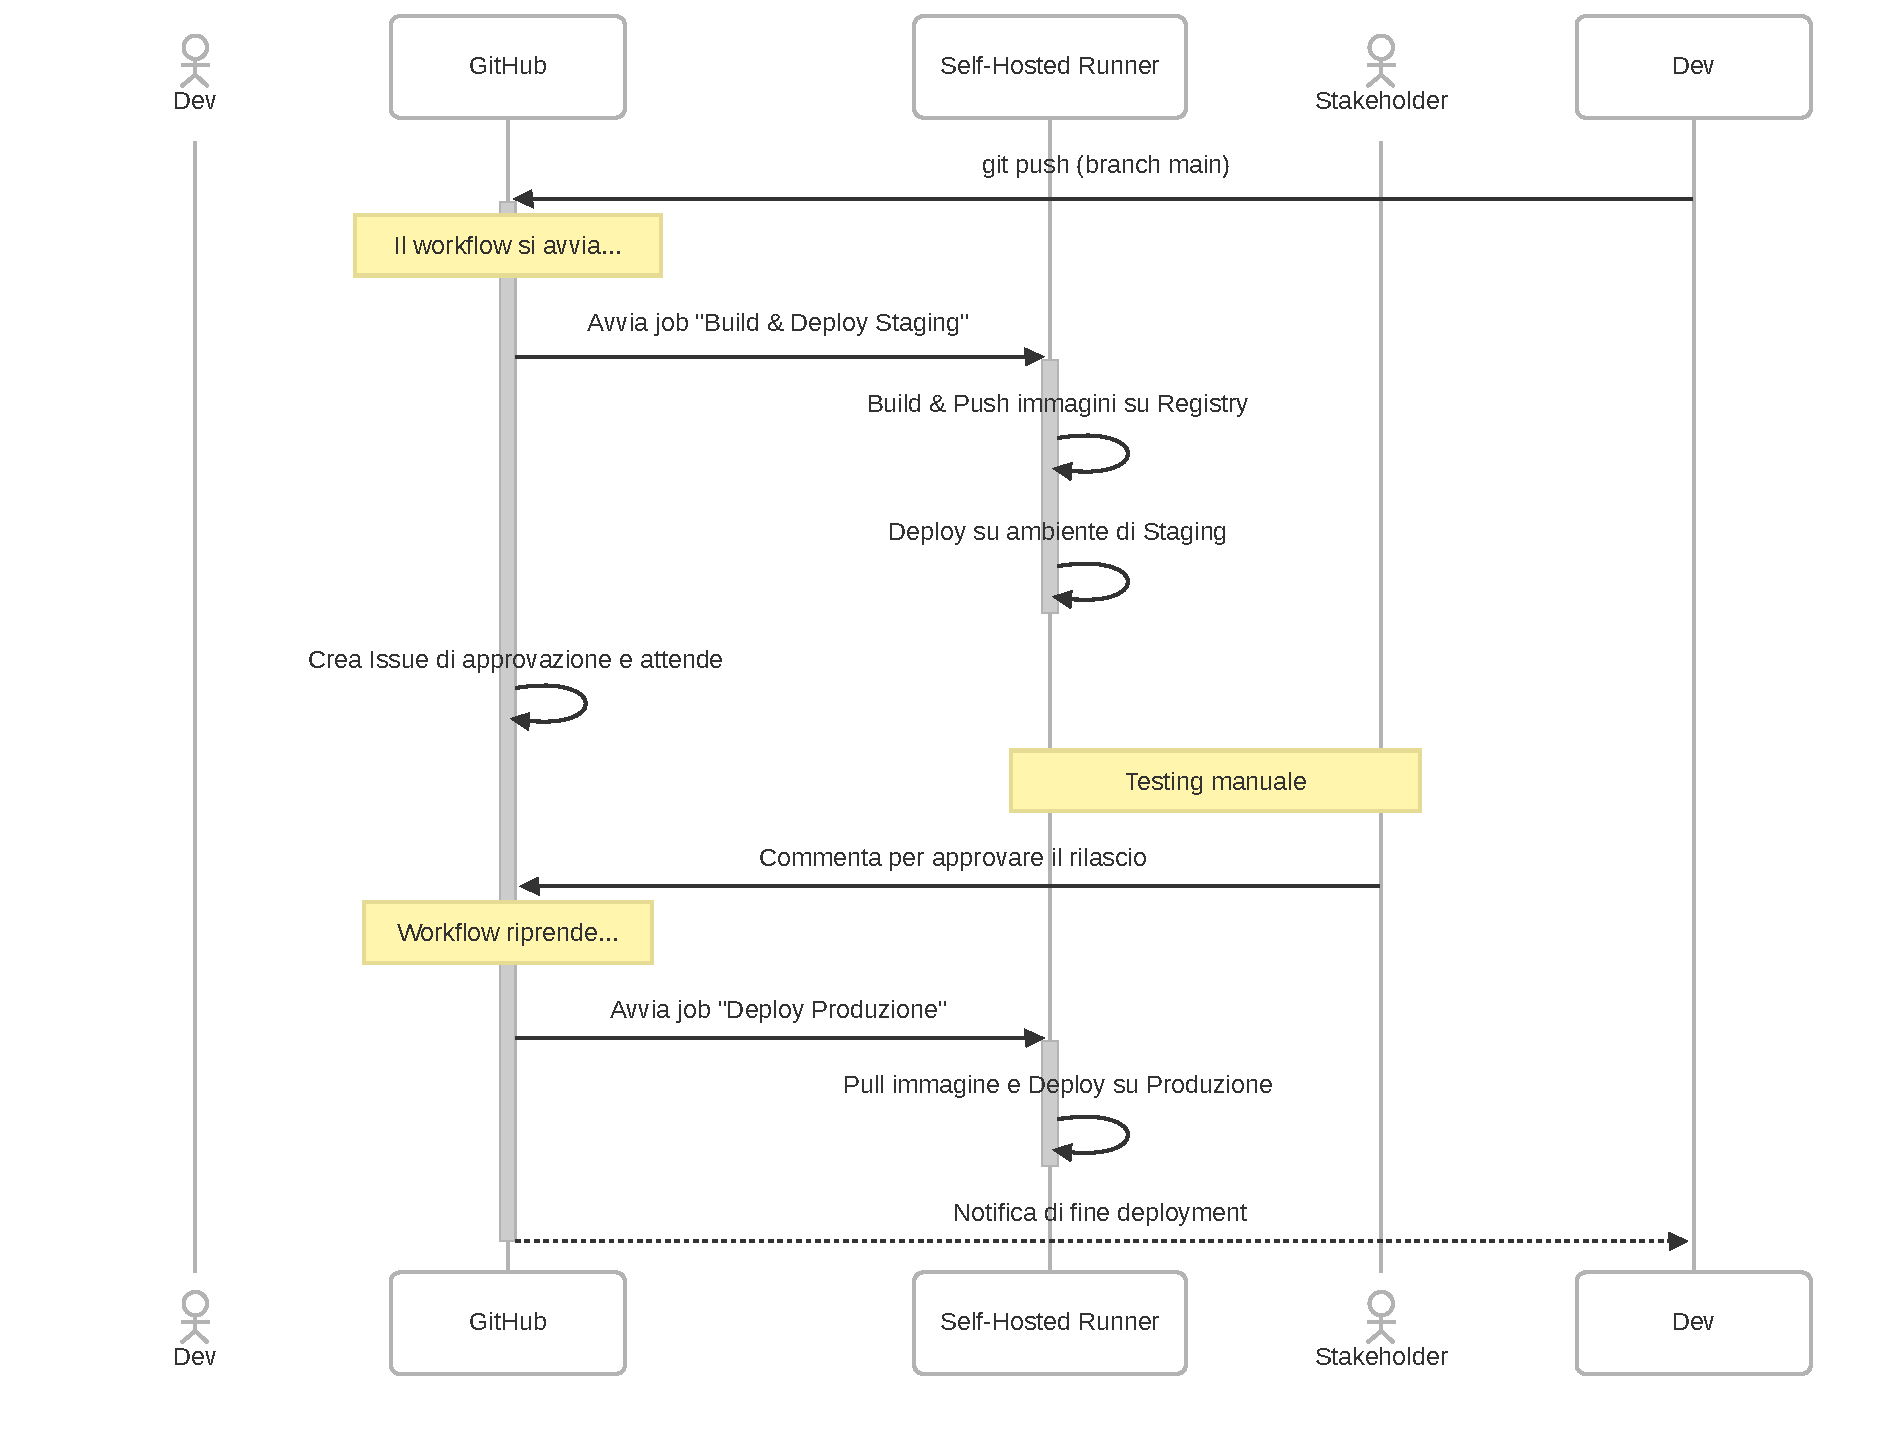
\includegraphics[width=\textwidth]{figures/pipeline_sequence.pdf}
    \caption{Diagramma che illustra il flusso di Continuous Integration e Continuous Deployment, dal push su Git al deployment sul server.}
    \label{fig:ci_cd_diagram}
\end{figure}



\chapter{Conclusioni e Sviluppi Futuri}
\label{chap:conclusioni}

Dal punto di vista pratico, l'obiettivo è stato pienamente raggiunto. È stata sviluppata e rilasciata un'applicazione web full-stack, basata su un'architettura moderna che gode dell'implementazione di un robusto flusso di autenticazione. Il successo e la stabilità della soluzione sono testimoniati dalla sua adozione in ambiente di piena produzione da parte di clienti di calibro internazionale come Telefónica e T-Mobile USA.

Dal punto di vista accademico e formativo, il progetto ha rappresentato un'opportunità unica di lavoro indipendente, fornendo piena libertà per quanto riguarda la metodologia di sviluppo e gran parte della progettazione.

In virtù della sua natura di "soluzione ponte", progettata per colmare un vuoto funzionale fino al rilascio della nuova piattaforma aziendale, e del pieno raggiungimento degli obiettivi prefissati, non sono previste evoluzioni sostanziali del software. Il suo ciclo di vita si conclude con successo con l'attuale versione in produzione, avendo adempiuto al suo scopo strategico.


\backmatter


\bibliographystyle{alpha}
\bibliography{bibliography}

\begin{acknowledgements}
    Optional. Max 1 page.
\end{acknowledgements}

\end{document}
